%% Template originaly created by Karol Kozioł (mail@karol-koziol.net) and modified for ShareLaTeX use

\documentclass[a4paper,13pt]{article}
\usepackage[linesnumbered,algoruled,boxed,lined]{algorithm2e}
\usepackage{multirow}
\usepackage[T1]{fontenc}
\usepackage[utf8]{inputenc}
\usepackage{graphicx}
\usepackage{xcolor}
\renewcommand\familydefault{\rmdefault}
\usepackage{tgheros}

\usepackage{amsmath,amssymb,amsthm,textcomp}
\usepackage{enumerate}
\usepackage{multicol}
\usepackage{tikz}
\usepackage[utf8]{vietnam}
\usepackage[unicode]{hyperref}
\usepackage{mathtools}
\usepackage[]{mdframed}

% draw a frame around given text
\newcommand{\framedtext}[1]{%
\par%
\noindent\fbox{%
    \parbox{\dimexpr\linewidth-2\fboxsep-2\fboxrule}{#1}%
}%
}
\newcommand\Myperm[2][^n]{\prescript{#1\mkern-2.5mu}{}P_{#2}}
\newcommand\Mycomb[2][^n]{\prescript{#1\mkern-0.5mu}{}C_{#2}}
\usepackage{geometry}
\geometry{total={210mm,297mm},
left=25mm,right=25mm,%
bindingoffset=0mm, top=22mm,bottom=25mm}

\linespread{1.3}

\newcommand{\linia}{\rule{\linewidth}{0.5pt}}

% custom theorems if needed
\newtheoremstyle{mytheor}
    {1ex}{1ex}{\normalfont}{0pt}{\scshape}{.}{1ex}
    {{\thmname{#1 }}{\thmnumber{#2}}{\thmnote{ (#3)}}}

\theoremstyle{mytheor}
\newtheorem{defi}{Definition}

% my own titles
\makeatletter
\renewcommand{\maketitle}{
\begin{center}
\vspace{2ex}
{\huge \textsc{\@title}}
\vspace{1ex}
\\
\linia\\
\@author \hfill \@date
\vspace{4ex}
\end{center}
}
\makeatother
%%%

% custom footers and headers
\usepackage{fancyhdr}
\setlength{\headheight}{20pt}
\pagestyle{fancy}
\fancyhead{} % clear all header fields
\fancyhead[L]{
 \begin{tabular}{rl}
    \begin{picture}(15,10)(0,0)
    \put(0,-8){
\includegraphics[width=8mm, height=8mm]{hcmut.png}}
    %\put(0,-8){\epsfig{width=10mm,figure=hcmut.eps}}
   \end{picture}&
	%
\includegraphics[width=8mm, height=8mm]{hcmut.png} & %
	\begin{tabular}{l}
		\textbf{\bf \ttfamily Ho Chi Minh City, University of Technology}\\
		\textbf{\bf \ttfamily Department of Computer Science and Engineer}
	\end{tabular} 	
 \end{tabular}
}
\fancyhead[R]{
	\begin{tabular}{l}
		\tiny \bf \\
		\tiny \bf 
	\end{tabular}  }
\fancyfoot{} % clear all footer fields
\fancyfoot[L]{\scriptsize \ttfamily Nghiên cứu phát triển kỹ thuật đếm số phần tử trên dòng dữ liệu}
\rfoot{Trang \thepage}
\renewcommand{\headrulewidth}{0.2pt}
\renewcommand{\footrulewidth}{0.2pt}
%

\usepackage{xcolor}
\definecolor{block-gray}{gray}{0.85}

\usepackage{environ}

\NewEnviron{myblock}
{
    \colorbox{block-gray}
    {
        \parbox{\dimexpr\linewidth-2\fboxsep\relax}
        {
            \bigbreak
            \addtolength{\leftskip}{4mm}
            \addtolength{\rightskip}{4mm}
            \BODY
        }
    }
}
\renewcommand{\quote}{\myblock}
\renewcommand{\endquote}{\endmyblock}
% code listing settings
\usepackage{listings}
\lstset{
    language=Python,
    basicstyle=\ttfamily\small,
    aboveskip={1.0\baselineskip},
    belowskip={1.0\baselineskip},
    columns=fixed,
    extendedchars=true,
    breaklines=true,
    tabsize=4,
    prebreak=\raisebox{0ex}[0ex][0ex]{\ensuremath{\hookleftarrow}},
    frame=lines,
    showtabs=false,
    showspaces=false,
    showstringspaces=false,
    keywordstyle=\color[rgb]{0.627,0.126,0.941},
    commentstyle=\color[rgb]{0.133,0.545,0.133},
    stringstyle=\color[rgb]{01,0,0},
    numbers=left,
    numberstyle=\small,
    stepnumber=1,
    numbersep=10pt,
    captionpos=t,
    escapeinside={\%*}{*)}
}
%%%----------%%%----------%%%----------%%%----------%%%

\begin{document}

\begin{titlepage}
\begin{center} {\textbf{ĐẠI HỌC QUỐC GIA TP. HỒ CHÍ MINH}
}

{\textbf{TRƯỜNG ĐẠI HỌC BÁCH KHOA}
}

{\textbf{KHOA KHOA HỌC VÀ KỸ THUẬT MÁY TÍNH }
}

{\textbf{---------------------------------------}}

\end{center}

\vspace{1cm}

\begin{figure}[h!]
\begin{center}

\includegraphics[width=3cm]{hcmut.png}
\end{center}
\end{figure}

\vspace{2cm}


\begin{center}
\begin{tabular}{c}
\multicolumn{1}{c}{\textbf{\Large NGHIÊN CỨU PHÁT TRIỂN KỸ THUẬT ĐẾM SỐ PHẦN TỬ TRÊN DÒNG DỮ LIỆU}}
\vspace{2cm}
\\
\multicolumn{1}{c}{\textbf{\Large LUẬN VĂN THẠC SĨ}}


~~\\

\\
\multicolumn{1}{l}{\textbf{{\Large}}}\\
\\
\textbf{{\Large}}\\

\\
\\

\end{tabular}
\end{center}

\vspace{1cm}

\begin{table}[h]
\begin{tabular}{rrl}
\hspace{5.1cm} 
&\textit{Học viên: } & \textbf{LÊ ANH QUỐC}\\
&\textit{ID: } & \textbf{2070428}\\

\end{tabular}
\end{table}
\vspace{3cm}
\begin{center}
{\footnotesize HỒ CHÍ MINH CITY}
\end{center}
\end{titlepage}

\begin{titlepage}
\begin{center} {\textbf{ĐẠI HỌC QUỐC GIA TP. HỒ CHÍ MINH}
}

{\textbf{TRƯỜNG ĐẠI HỌC BÁCH KHOA}
}

{\textbf{KHOA KHOA HỌC VÀ KỸ THUẬT MÁY TÍNH }
}

{\textbf{---------------------------------------}}

\end{center}

\vspace{1cm}

\begin{figure}[h!]
\begin{center}

\includegraphics[width=3cm]{hcmut.png}
\end{center}
\end{figure}

\vspace{2cm}


\begin{center}
\begin{tabular}{c}
\multicolumn{1}{c}{\textbf{\Large NGHIÊN CỨU PHÁT TRIỂN KỸ THUẬT ĐẾM SỐ PHẦN TỬ TRÊN DÒNG DỮ LIỆU}}
\vspace{2cm}
\\
\multicolumn{1}{c}{\textbf{\Large LUẬN VĂN THẠC SĨ}}

\vspace{0.5cm}
\\
\multicolumn{1}{c}{\text{\small NGÀNH: KHOA HỌC MÁY TÍNH }}
\vspace{0.5cm}
\\
\multicolumn{1}{c}{\text{\small MÃ NGÀNH: \textbf{8480101} }}
\vspace{1cm}
\\
\multicolumn{1}{c}{\textbf{\small NGƯỜI HƯỚNG DẪN KHOA HỌC }}
~~\\
\multicolumn{1}{c}{\textbf{\small PGS. TS. THOẠI NAM
 }}

\\
\\

\\
\\

\end{tabular}
\end{center}

\vspace{1cm}

\begin{table}[h]
\begin{tabular}{rrl}
\hspace{5.6cm} 
&\textit{Học viên: } & \textbf{lÊ ANH QUỐC}\\
&\textit{ID: } & \textbf{2070428}\\

\end{tabular}
\end{table}
\vspace{1cm}
\begin{center}
{\footnotesize HỒ CHÍ MINH CITY}
\end{center}
\end{titlepage}

%%%----------%%%----------%%%----------%%%----------%%%


%\thispagestyle{empty}

\renewcommand{\contentsname}{Content}
\newpage
\vspace{1cm}
\tableofcontents
\newpage
\section{GIỚI THIỆU ĐỀ TÀI, MỤC TIÊU VÀ ĐỐI TƯỢNG NGHIÊN CỨU}
\subsection{Tính cấp thiết và lý do chọn đề tài}
\hspace{2em}Ngày nay, các ứng dụng và dịch vụ trực tuyến đóng vai trò ngày càng quan trọng trong cuộc sống của con người. 
Chúng ta sử dụng mạng xã hội để kết nối với bạn bè và chia sẻ thông tin, mua sắm trực tuyến để tiết kiệm thời gian và tiền bạc, 
hay xem phim và chơi game trực tuyến để giải trí. Để đánh giá hiệu quả hoạt động của các ứng dụng và dịch vụ này, 
một trọng những chỉ số quan trọng nhất là số lượng người dùng hoạt động Distinct Active Users (DAU).

Việc theo dõi số lượng người dùng hoạt động trong một khoảng thời gian nhất định trên một dòng dữ liệu (data stream) 
là một yêu cầu quan trọng đối với nhiều ứng dụng và dịch vụ trực tuyến, hiệu quả của các chiến dịch marketing, 
và hỗ trợ ra quyết định kinh doanh. Ví dụ, trong các ứng dụng mạng xã hội, số lượng người dùng hoạt động cho thấy mức độ tương tác 
và sự quan tâm của người dùng đối với nền tảng. Trong các dịch vụ thương mại điện tử, số lượng người dùng hoạt động cho thấy hiệu quả 
và các chiến dịch quảng cáo và khuyến mãi. Tuy nhiên, việc đếm số lượng DAU không phải là một nhiệm vụ đơn giản, đặc biệt là khi dữ liệu lớn 
và tốc độ truy cập cao. Các phương pháp truyền thống như lưu trữ và truy vấn trực tiếp vào cơ sở dữ liệu có thể gặp nhiều hạn chế về hiệu suất 
và khả năng mở rộng.

Trong nhiều trường hợp, cần phải tổng hợp số lượng DAU trên nhiều streams hoặc services khác nhau. Việc này giúp có được bức tranh toàn cảnh về hoạt động của người dùng trên toàn hệ thống, từ đó đưa ra các phân tích và đánh giá chính xác hơn. Ví dụ, trong hệ thống thương mại điện tử, cần tổng hợp số lượng DAU từ các trang web, ứng dụng di động và API khác nhau để có được số lượng người dùng hoạt động thực tế trên toàn hệ thống. Tuy nhiên, việc tổng hợp dữ liệu từ nhiều nguồn khác nhau có thể gặp thách thức về đồng bộ hóa dữ liệu, xử lý dữ liệu bị thiếu hoặc lỗi, và đảm bảo tính nhất quán của kết quả. 

Ngoài ra, có thể cần phải đếm DAU trên nhiều đoạn khác nhau trong một stream, hoặc nhiều streams khác nhau. Việc này giúp phân tích chi tiết hơn hoạt động của người dùng theo thời gian, theo khu vực hoặc theo tiêu chí khác. Ví dụ, trong một ứng dụng phát trực tiếp, cần đếm số lượng người dùng hoạt động theo từng giờ hoặc từng phân đoạn chương trình để đánh giá mức độ quan tâm của người xem. Tuy nhiên, việc phân chia và xử lý dữ liệu theo nhiều đoạn có thể làm tăng độ phức tạp của thuật toán và ảnh hưởng đến hiệu suất của hệ thống. Do đó, cần phải có một giải pháp đếm số lượng phần tử trên dòng dữ liệu đạt hiệu suất cao và tin cậy, từ đó có thể ứng dụng rộng rãi trong các hệ thống khác nhau như mạng xã hội, thương mại điện tử, chương trình phát trực tiếp, hệ thống giám sát và hệ thống giao thông thông minh.

\subsection{Mục tiêu nghiên cứu }
\subsubsection{Phát triển thuật toán để đếm DAU trên một dòng dữ liệu (data stream):}
Thiết kế thuật toán sử dụng HyperLogLog để đếm DAU trên một khung thời gian trên một stream với độ chính xác cao và hiệu quả tốt. Ví dụ, đếm số lượng users đăng nhập vào hệ thống trong 5 phút trước, 1 giờ trước, 1 ngày trước hay 1 tháng trước.
\subsubsection{Mở rộng thuật toán để đếm DAU trong một khoảng thời gian trên nhiều streams:}
\subsubsection{Phát triển một thuật toán để đếm DAU trên nhiều khung thời gian và trên nhiều streams hoặc services khác nhau:}
Phát triển phương pháp và công cụ giám sát: Mục tiêu chính là thiết kế và phát triển các phương pháp và công cụ giám sát pin hiệu quả trên xe điện. Điều này bao gồm việc xác định các thông số quan trọng cần được giám sát như trạng thái sạc, nhiệt độ, dòng điện và điện áp của pin. Công cụ giám sát cần có khả năng thu thập, xử lý và hiển thị dữ liệu pin một cách dễ dàng và đáng tin cậy.\\
Phân tích và đánh giá hiệu suất hoạt động của pin: Mục tiêu là phân tích và đánh giá hiệu suất hoạt động của pin trên xe điện. Điều này có thể bao gồm việc theo dõi và ghi nhận các thông số pin trong quá trình vận hành, phân tích các dữ liệu thu thập được để đánh giá hiệu suất sạc, xả và tổn thất năng lượng. Mục tiêu cuối cùng là tối ưu hóa sử dụng năng lượng và kéo dài tuổi thọ pin thông qua các biện pháp quản lý phù hợp.\\
Phát hiện sớm các vấn đề và rủi ro: Mục tiêu là phát triển các thuật toán và phương pháp giám sát pin để phát hiện sớm các vấn đề và rủi ro tiềm ẩn. Điều này bao gồm việc xây dựng các mô hình dự đoán và cảnh báo để nhận biết các tình huống nguy hiểm như quá nhiệt, quá dòng, hao mòn pin nhanh chóng và các lỗi khác. Mục tiêu là nâng cao mức độ an toàn và độ tin cậy của hệ thống pin trên xe điện.\\
Nghiên cứu và ứng dụng công nghệ mới: Mục tiêu cuối cùng là nghiên cứu và áp dụng các công nghệ mới để cải thiện giám sát pin trên xe điện. Điều này có thể bao gồm việc sử dụng các cảm biến tiên tiến, hệ thống ghi dữ liệu thông minh, trí tuệ nhân tạo và học máy để tăng cường khả năng giám sát và dự đoán của hệ thống. Mục tiêu là tạo ra một hệ thống giám sát pin tiên tiến, đáng tin cậy và hiệu quả cho xe điện.

\subsection{Giới hạn và đối tượng nghiên cứu }
\subsubsection{Giới hạn}
Độ chính xác và độ tin cậy: Một trong những thách thức chính là đảm bảo độ chính xác và độ tin cậy của hệ thống giám sát pin trên xe điện. Các thông số pin cần được đo lường và giám sát một cách chính xác để đưa ra các quyết định đúng đắn và đảm bảo an toàn. Đồng thời, hệ thống giám sát phải đảm bảo tính tin cậy trong môi trường hoạt động khắc nghiệt và đảm bảo hoạt động liên tục của xe điện.\\
Quản lý dữ liệu: Việc giám sát pin trên xe điện có thể tạo ra lượng lớn dữ liệu, và việc quản lý và xử lý dữ liệu một cách hiệu quả là một thách thức. Cần phải xây dựng các phương pháp, công nghệ và hệ thống để thu thập, lưu trữ, xử lý và phân tích dữ liệu pin một cách hiệu quả và đáng tin cậy.
\subsubsection{Đối tượng nghiên cứu }
Đối tượng nghiên cứu của đề tài "Giám sát pin trên xe điện" là các yếu tố liên quan đến pin và hệ thống giám sát pin trên xe điện, nhằm tối ưu hóa hiệu suất, tuổi thọ và an toàn của pin trong hoạt động của xe điện.

\section{CÁC CÔNG TRÌNH NGHIÊN CỨU LIÊN QUAN }
- \textbf{Battery Management Systems in Electric and Hybrid Vehicles} – [1] Công trình này tập trung vào khái niệm và chức năng của hệ thống quản lý pin (BMS) trong xe điện và hybrid. Nó giới thiệu các yếu tố quan trọng trong việc giám sát pin như trạng thái sạc, nhiệt độ, điện áp và dòng điện, cũng như các chiến lược quản lý pin để tăng hiệu suất và tuổi thọ của pin.\\

- \textbf{State of Charge Estimation of Lithium-Ion Batteries in Electric Vehicles: A Review} – [2] Công trình này tập trung vào việc ước lượng trạng thái sạc của pin Lithium-Ion trong xe điện. Nó xem xét các phương pháp và thuật toán được sử dụng để ước lượng trạng thái sạc và đánh giá hiệu suất của chúng.\\

- \textbf{Real-Time State of Health Estimation for Lithium-Ion Batteries in Electric Vehicles} – [3] Công trình này tập trung vào ước lượng trạng thái sức khỏe (SOH) của pin Lithium-Ion trong xe điện. Nó đề xuất một phương pháp ước lượng SOH dựa trên phân tích dữ liệu pin thời gian thực và sử dụng mô hình dự đoán để đánh giá tuổi thọ còn lại của pin.\\

- \textbf{Data-Driven Fault Diagnosis and Prognosis of Lithium-Ion Batteries in Electric Vehicles} – [4] Công trình này tập trung vào việc chẩn đoán và tiên đoán lỗi cho pin Lithium-Ion trong xe điện. Nó sử dụng phương pháp dựa trên dữ liệu để phân tích và phát hiện các lỗi potentiostatic, impedance và voltage của pin, cung cấp thông tin quan trọng để dự đoán tuổi thọ và hiệu suất của pin.\\

- \textbf{Intelligent Battery Management and Control for Electric Vehicles} – [5] Công trình này tập trung vào nghiên cứu về quản lý và điều khiển pin thông minh cho xe điện. Nó đề xuất một hệ thống BMS thông minh sử dụng công nghệ trí tuệ nhân tạo và học máy để giám sát và dự đoán trạng thái pin, tối ưu hóa sử dụng năng lượng và quản lý tuổi thọ của pin.\\

\section{HyperLogLog}
The \textit{cardinality} estimation problem is a task to find the number of distinct
elements in a dataset where duplicates are present. Traditionally, to
determine the exact cardinality of a set, classical methods build a list
of all elements and use sorting and search to avoid listing elements
multiple times. Counting the number of elements in that list gives the accurate
number of the unique elements, but it has a time complexity of O(N.logN), where
N is the number of all elements including duplicates, and requires auxiliary 
linear memory, that is unlikely to be feasible for Big Data applications that
operate huge datasets of large cardinalities.
\begin{mdframed}
   \textbf{Ví dụ 3.1: Số lượng khách truy cập}\\
    Một trong những chỉ số KPI quý giá cho bất kỳ trang web nào là số lượng khách truy cập duy nhất đã ghé thăm trong một khoảng thời gian cụ thể. 
    Để đơn giản, chúng ta giả định rằng khách truy cập duy nhất sử dụng các địa chỉ IP khác nhau, do đó chúng ta cần tính toán số lượng địa chỉ IP 
    duy nhất mà theo giao thức Internet IPv6 được biểu diễn bằng chuỗi 128-bit. Liệu đây có phải là một nhiệm vụ dễ dàng không? 
    Chúng ta có thể chỉ sử dụng các phương pháp cổ điển để đếm số lượng một cách chính xác không? Điều này phụ thuộc vào sự phổ biến của trang web.\\
    Xem xét thống kê lưu lượng cho tháng 3 năm 2017 của ba trang web bán lẻ phổ biến nhất tại Hoa Kỳ: \textit{amazon.dot, ebay.com} và 
    \textit{walmart.com}. Theo SimilarWeb, số lần truy cập trung bình đến các trang web đó là khoảng 1,44 tỷ và số lượng trang xem trung bình 
    mỗi lần truy cập là 8,24. Do đó, thống kê cho tháng 3 năm 2017 bao gồm khoảng 12 tỷ địa chỉ IP với mỗi địa chỉ có 128-bit, tức là tổng 
    kích thước là 192 GB.\\
    Nếu chúng ta giả định rằng mỗi 10 người trong số những khách truy cập đó là duy nhất, chúng ta có thể mong đợi số lượng phần tử 
    trong tập hợp đó là khoảng 144 triệu và bộ nhớ cần thiết để lưu trữ danh sách các phần tử duy nhất là 23 GB.
\end{mdframed}
\break
Another example illustrates the challenge of cardinality estimation for\\
scientific researchers.
\begin{mdframed}
    \textbf{Example 3.2: DNA analysis (Giroire, 2016)}\\
    One of the long-standing tasks in human genome research is to study
    correlation in DNA sequences. DNA molecules include two paired strands,
    each made up of four chemical DNA-base units, marked A (adenine),
    G (guanine), C (cytosine), and T (thymine). The human genome contains
    about 3 billion such base pairs. Sequenceing means determining the exact
    order of the base pairs in a segment of DNA.\\
    From a mathematical point of view, a DNA sequence can be considered
    a string of symbols A, G, C, T which can be as long as you want, and we
    can consider them as an example of a potentially infinite dataset.\\
    The correlation measuring problem can be formulated as a task of
    determining the number of distinct substrings of some fixed size in a piece
    of DNA. The idea is that a sequence with a few distinct substrings is 
    more correlated than a sequence of the same size but with more distinct
    substrings.\\
    Such experiments demand multiple runs on many huge files and to speed
    up the research they require only limited or even constant memory and
    small execution time, which is unfeasible with exact counting algorithms.
\end{mdframed}
Thus, the possible gains of the accurate cardinality estimation are
neglected by large time processing and memory requirements. Big Data
applications shell use more practical approaches, mostly based on various
probabilistic algorithms, even if they can provide only approzimated answers.\\
\vspace{0.5cm}
\begin{quote}
    While processing data, it is important to understand the size of the dataset
    and the number of possible distinct elements.\\
    Consider the potentially infinite sequence of 1-letter string a, d, s, ...,
    which is based on letters from the English alphabet. The cardinality can be
    easily estimated and it is upper bounded by the number of letters, which
    is 26 in the modern English language. Obviously, in this case, there is
    no need to apply any probabilistic approach and a naive dictionary-based
    solution of exact cardinality calculation works very well.\\
\end{quote}
\indent To approach the cardinality problem, many of the popular probabilistic
methods are influenced by the ideas of the Bloom filter algorithm, they
operate hash values of elements, then observe common patterns in their
distribution, and make reasoned \textquotedblleft\textit{guesses}\textquotedblright 
\space about the number of unique elements without the need to store all of them.
\subsection{Linear Counting}
As a first probabilistic approach to the cardinality problem, we consider
the linear-time probabilistic counting algorithm, the \textit{Linear Counting}
algorithm. The original ideas were proposed by Morton Astrahan, Mario Schkolnick,
and Kyu-Young Whang in 1987 [As87] and the practical algorithm was published
by Kyu-Young Whang, Brad Vander-Zanden, and Howard Taylor in 1990 [Wh90].\\
\indent The immediate improvement to the classical exact methods was to
hash elements with some hash function \textit{h}, which out-of-the-box can
eliminate duplicates without the need to sort elements with a payout of
introducing some probability of error due to possible hash collisions
(we cannot distinguish duplicates and \textquotedblleft accidental duplicates\textquotedblright).
Thus, using such a hash table, only a proper scan procedure is required to implement
a simple algorithm that already outperforms the classical approach.\\
\indent However, for datasets with huge cardinalities, such hash tables could
be quite large and require memory that grows linearly with the number
of distinct elements in the set. For systems with limited memory, it
will require disk or distributed storage at some point, which drastically
reduces the benefits of hash tables due to slow disk or network access.\\
\indent Similar to the Bloom filter idea, to work-around such an issue,
the Linear Counting algorithm doesn't store the hash values themselves,
but instead their corresponding bits, replacing the hash table with a bit
array LINEARCOUNTER of the length \textit{m}. It is assumed that \textit{m} still is
proportional to the expected number of distinct elements \textit{n}, but requires
only 1 bit per element which is feasible for most cases.\\
\indent In the beginning, all bits in LINEARCOUNTER are equal to zero. To
add a new element \textit{x} into such a data structure, we compute its hash
value \textit{h(x)} and set the corresponding bit to one in the counter.\\\\
\vspace{0.5cm}
\begin{algorithm}[H]
    \DontPrintSemicolon
    \LinesNumberedHidden
    \caption[]{Adding element to the Linear counter}
    \KwIn{Element $x \in D$}
    \KwIn{Linear counter with hash function $h$}
    $j \gets h(x)$\;
    \If{$LINEARCOUNTER[j] == 5$}
    {
        $LINEARCOUNTER[j]\gets 1$
    }
\end{algorithm}
\indent Since only one hash function \textit{h} is used, we can expect many additional
hard collisions when two different hash values set the same bit in the array.
Thus, the exact (or even near-exact) number of distinct elements can no
longer be directly obtained from such a sketch.\\
\indent The idea of the algorithm leads to distributing elements into buckets
(bits indexed by hash values) and keeps a LINEARCOUNTER bit array 
indicating which buckets are hit. Observing the number of hits in the array
leads to the estimate of the cardinality.\\
\indent In the first step of the Linear Counting algorithm, we build our
LINEARCOUNTER data structure as is shown in Algorighm 1. Having
such a sketch, the cardinality can be estimated using the observed
fraction of empty bits \textbf{V} by the formula:\\
\begin{equation}
    n \approx -m\cdot\ln V \tag{$3.1$}
\end{equation}
\indent We see clearly now how collisions impact on the cardinality estimation
in the Linear Counting algorithm -- each collision reduces the number
of bits that have to bet set, making the observed fraction of unset bits
bigger than the real value. If there were no hash collisions, the final
count of set bits would be the desired cardinality. However, collisions
are unvoidable and the formula (3.1) actually gives an overestimation
of the exact cardinality and, since the cardinality is an integer value, we
prefer to round its result to the nearest smaller integer.\\
\indent Thus, we can formulate the complete counting algorithm as bellow.\\
\vspace{0.5cm}
\begin{algorithm}[H]
    \DontPrintSemicolon
    \LinesNumberedHidden
    \caption[]{Estimating cardinality with Linear Counting}
    \KwIn{Dataset $ D $}
    \KwOut{Cardinality estimation}
    LINEARCOUNTER[j] $\gets 0$, $i = 0$ ... m $- $ 1\;
    \For{x $\in $ D} { LINEARCOUNTER.Add(e) }
    Z $\gets count_{i=1...m-1} (LINEARCOUNTER[i] = 0 $)\;
    \Return{$-m \cdot \ln(\frac{Z}{m})$}
\end{algorithm}
\begin{mdframed}
    \textbf{Example 3.3: Linear Counting algorithm}\\
    Consider a dataset that contains 20 names of capital cities extracted
    from recent news articles: \textbf{Berlin,} Berlin, \textbf{Paris,} Berlin,
    \textbf{Lisbon, Kiev,} Paris, \textbf{London, Rome, Athens, Madrid, Vienna,}
    Rome, Rome, Lisbon, Berlin, Paris, London, Kiev, \textbf{Washington.}\\
    For such small cardinalities (actual cardinality is 10) to have a standard
    error about 10\% we need to choose the length of the LINEARCOUNTER
    data structure at least as the expected number of unique elements, thus
    let's choose m$ = 2^4$. As the hash function $h$ with values in ${0,1,...,2^4-1}$
    we use a function based on 32-bit MurmurHash3 defined as
    \begin{equation}
        h(x) := MurmurHash3(x)\mod m,
      \end{equation}
    and cities hash values can be found in the table below.
\begin{center}
    \begin{tabular}{ |c|c| }
        \multicolumn{2}{}{} \\ \hline
        \textbf{City} & \textbf{h(City)} \\ \hline
        Athens & 12 \\
        Berlin & 7 \\
        Kiev & 13 \\
        Lisbon & 15 \\
        London & 14 \\
        \cline{1-2}
    \end{tabular}
    \hspace{0.5cm}
    \begin{tabular}{ |c|c| }
        \multicolumn{2}{}{}\\ \hline
        \textbf{City} & \textbf{h(City)} \\ \hline
        Madrid & 14 \\
        Paris & 8 \\
        Rome & 1 \\
        Vienna & 6 \\
        Washington & 11 \\
        \cline{1-2}
    \end{tabular}
\end{center}
As we can see, the cities \textbf{London} and \textbf{Madrid} share the same value, but
such colisions are expected and completely natural. The LINEARCOUNTER
data structure has the following view:
\begin{center}
    \begin{tabular}{p{0.4cm}p{0.4cm}p{0.4cm}p{0.4cm}p{0.4cm}p{0.4cm}p{0.4cm}p{0.4cm}p{0.4cm}p{0.4cm}p{0.4cm}p{0.4cm}p{0.4cm}p{0.4cm}p{0.4cm}p{0.4cm}}
        0 & 1 & 2 & 3 & 4 & 5 & 6 & 7 & 8 & 9 & 10 & 11 & 12 & 13 & 14 & 15 % Add bottom border to all rows
    \end{tabular}
    \begin{tabular}{|p{0.4cm}|p{0.4cm}|p{0.4cm}|p{0.4cm}|p{0.4cm}|p{0.4cm}|p{0.4cm}|p{0.4cm}|p{0.4cm}|p{0.4cm}|p{0.4cm}|p{0.4cm}|p{0.4cm}|p{0.4cm}|p{0.4cm}|p{0.4cm}|}
        \hline
        0 & 1 & 0 & 0 & 0 & 0 & 1 & 1 & 1 & 0 & 0 & 1 & 1 & 1 & 1 & 1 \\ \cline{1-16} % Add bottom border to all rows
    \end{tabular}
\end{center}
\vspace{0.2cm}
According to the Linear Counting algorithm, we calculate the fraction \textbf{V}
of empty bits in the LINEARCOUNTER:
\begin{equation}
    V = \frac{9}{16} = 0.5625
\end{equation}
and the estimated cardinality is
\begin{equation}
    n \approx -16\cdot \ln 0.5625 \approx 9.206,
\end{equation}
which is pretty close to th exact number 10.
\end{mdframed}
\subsection*{Properties}
If the hash function $h$ can be computed in a constant time (which is true
for the most popular hash function), the time to process every element is
a fixed constant O(N), where N is the total number of elements, including
duplicates. Thus, the algorithm has O(N) time complexity.\\
\indent As for many other probabilistic algorithm, there is a number of
parameters that can be runed to influence its performance.\\
\indent The expected accuracy of the estimation depends on the bit array
size $m$ and its ratio to the number of distinct elements $\alpha$ = $\frac{m}{n}$, called
the \textit{load factor}. Unless $\alpha$ $\geq$ $1$ ($m$ > $n$ is not practically interesting case),
there is non-zero probability $P_{full}$ that LINEARCOUNTER bit array
becomes full, called the $fill-up probability$, that fatally distorts
the algorithm and blows up the expression (3.1). The probability $P_{full}$
depends on the load factor and, consequently, on the size $m$ that should
be selected big enough to have the fill-up probability negligible.\\
\indent The standard error $\sigma$ is a measure of the variability of the estimate
provided by Linear Counting and there is a trade-off between it and
the bit array zise $m$. Descreasing the standard error results in more
precies estimates, but increase the require memory.\\\\
\begin{quote}
    \begin{center}
        \textbf{Table 3.1:} Trade-off between accuracy and bit array size\\
        \begin{tabular}{|*{3}{c|}}
            \hline
            \multirow{2}{*}{n} & \multicolumn{2}{c|}{\text{m}} \\ \cline{2-3} 
                    & $\sigma = 1\%$ & $\sigma = 10\%$ \\ \hline
            1000 & 5329 & 268 \\ \hline
            10000 & 7960 & 1709 \\ \hline
            100000 & 26729 & 12744 \\ \hline
            10000000 & 154171 & 100880 \\ \hline
            10000000 & 1096582 & 831809 \\ \hline
            100000000 & 8571013 & 7061760 \\ \hline
        \end{tabular}
    \end{center}
\end{quote}\\

The dependence on choosing $m$ is quite complex and has no analysis
solution. However, for a widely acceptable fill-up probabilistic $P_full = 0.7\%$
the algorithm authors have provided precomputed values that are given in Table 3.1
and can be used as references.

Since the fill-up probability is never zero, the bit array very rarely
becomes full and distorts Algorithm 3.2. When working with small
datasets, we can re-index all elements with a different hahs function or 
increase the size LINEARCOUNTER. Unfortunately, such solutions
won't work for huge datasets and, together with quite high time
complexity, require a search for alternatives.

However, Linear Counting performs very well when the cardinality
of the dataset being measured is not extreamly big and can be used to
improve other algorithm, developed to provide the best possible behavior
for huge cardinalities.

In the Linear Counting algorithm, the estimation of the cardinality
is approximately proportional to the exact value, this is why the term
\textquotedblleft linear\textquotedblright\space is used. In the next section, we consider an alternative algorithm
that could be classified as \textquotedblleft logarithmi\textquotedblright\space counting since it is based on
estimations that logarithms of the true cardinality.
\subsection{Probabilistic Counting}
One of the counting algorithms that is based on the idea of observing
commom patterns in hashed representations of indexed elements is a class
of \textit{Probabilistic Counting} algorithm is invented by Philippe Flajolet and
G. Nigel Martin in 1985 [Fl85].

As asual, every element is pre-processed by applying a hash function $h$
that transforms elements into integers sufficiently uniformaly distributed
over a scala range ${0, 1,...,2^M - 1}$ or, quivalently, over the set of
binary $strings^2$ of length M:

\[h(x) = i = \sum_{k=0}^{M-1} i_k\cdot 2^k := (i_0i_1...i_{M-1})_2, i_k \in \{0,1\}.\]

Flajolet and Martin noticed that patterns:
\[0^k1 := \overbrace{00...0}^{\text{k times}}1\]
should appear in such binary strings with probability $2^{-(k+1)}$ and, if
recorded for each indexed element, can play the role of a cardinality
estimator.

Every pettern can be associated with its index, called $rank$, that is
calculated by the formula:
\[
    rank(i)=\left\{
                \begin{array}{ll}
                    \min\limits_{i_k\neq 0}, \indent\text{for } i > 0,\\
                    M\indent\indent\text{for } i = 0
                \end{array}
            \right.
\]
and simply equivalent to the left-most position of 1, known as the least
significant 1-bit position.
\begin{mdframed}
    \textbf{Example 3.4: Rank calculation}\\
    Consider an 8-bit long integer number 42 that has the following binary
    representation using the \textquotedblleft LSB 0\textquotedblright numbering scheme:
    \[
        42 = 0\cdot2^0+1\cdot2^1+0\cdot2^2+1\cdot2^3+0\cdot2^4+1\cdot2^5+0\cdot2^6+0\cdot2^7 = (0\textbf{1}010100)_2 .
    \]
    Thus, the ones appear at positions 1, 3, and 5, therefore, accroding to
    the definition (3.2), the rank(42) is equal to:
    \[rank(42) = \min(1,3,5) = 1.\]
\end{mdframed}
The accurences of the $0^k 1$ pattern, or simply $rank(\cdot) = k$, in binary
representations of hash values of each indexed element, can be compactly
stored in a simple data structure COUNTER, also known as a FM Sketch,
that is represented as a bit array of length M.

At the start, all bits in COUNTER are equal to zero. When we need to
add a new element $x$ into the data structure, we compute its hash value
using the hash function $h$, then calculate rank(x) and set
the corresponding bit to one in the array, as stated in the algorithm
below.\\
\begin{algorithm}[H]
    \DontPrintSemicolon
    \LinesNumberedHidden
    \caption[]{Adding element to simple counter}
    \KwIn{Element $x \in D$}
    \KwIn{Simple counter with hash function $h$}
    $j \gets rank(h(x))$\;
    \If{$LINEARCOUNTER[j] == 0$}
    {
        $LINEARCOUNTER[j]\gets 1$
    }
\end{algorithm}
\vspace{0.4cm}
In this way, the one in the COUNTER at some position $j$ means that
the pattern $0^i 1$ has been observed at least once amongst the hashed
values of all indexed elements.
\begin{mdframed}
    \textbf{Example 3.5: Build a simple counter}\\
    Consider the same datasets as in Example 3.3 that contains 20 names
    of capital cities extracted from recent news articales: \textbf{Berlin,} Berlin, \textbf{Paris,} Berlin,
    \textbf{Lisbon, Kiev,} Paris, \textbf{London, Rome, Athens, Madrid, Vienna,}
    Rome, Rome, Lisbon, Berlin, Paris, London, Kiev, \textbf{Washington.}\\
    As the hash function $h$ we can use 32-bit MurmurHash3, that maps elements
    to values from ${0,1,...,2^{32} - 1}$, therefore we can use simple counter
    COUNTER of length M = 32. Using the hash values already computed in 
    Example 3.3 and the definition (3.2), we calculate ranks for each element:
    \begin{center}
        \begin{tabular}{ |c|c|c| }
            \multicolumn{3}{}{} \\ \hline
            \textbf{City} & \textbf{h(City)} & \textbf{rank} \\ \hline
            Athens & 4161497820 & 2 \\
            Berlin & 3680793991 & 0 \\
            Kiev & 3491299693 & 0 \\
            Lisbon & 629555247 & 0 \\
            London & 3450927422 & 1 \\
            Rome & 50122705 & 0 \\
            Vienna & 3271070806 & 1 \\
            Washington & 4039747979 & 0\\
            \cline{1-3}
        \end{tabular}
    \end{center}
    Thus, the COUNTER has following form:
    \begin{center}
        \begin{tabular}{p{0.4cm}p{0.4cm}p{0.4cm}p{0.4cm}p{0.4cm}p{0.4cm}p{0.4cm}p{0.4cm}p{0.4cm}p{0.4cm}p{0.4cm}p{0.4cm}p{0.4cm}p{0.4cm}p{0.4cm}p{0.4cm}}
            0 & 1 & 2 & 3 & 4 & 5 & 6 & 7 & 8 & 9 & 10 & 11 & 12 & 13 & 14 & 15 % Add bottom border to all rows
        \end{tabular}
        \begin{tabular}{|p{0.4cm}|p{0.4cm}|p{0.4cm}|p{0.4cm}|p{0.4cm}|p{0.4cm}|p{0.4cm}|p{0.4cm}|p{0.4cm}|p{0.4cm}|p{0.4cm}|p{0.4cm}|p{0.4cm}|p{0.4cm}|p{0.4cm}|p{0.4cm}|}
            \hline
            1 & 1 & 1 & 1 & 0 & 0 & 0 & 0 & 0 & 0 & 0 & 0 & 0 & 0 & 0 & 0 \\ \cline{1-16} % Add bottom border to all rows
        \end{tabular}
        \begin{tabular}{p{0.4cm}p{0.4cm}p{0.4cm}p{0.4cm}p{0.4cm}p{0.4cm}p{0.4cm}p{0.4cm}p{0.4cm}p{0.4cm}p{0.4cm}p{0.4cm}p{0.4cm}p{0.4cm}p{0.4cm}p{0.4cm}}
            16 & 17 & 18 & 19 & 20 & 21 & 22 & 23 & 24 & 25 & 26 & 27 & 28 & 29 & 30 & 31 % Add bottom border to all rows
        \end{tabular}
        \begin{tabular}{|p{0.4cm}|p{0.4cm}|p{0.4cm}|p{0.4cm}|p{0.4cm}|p{0.4cm}|p{0.4cm}|p{0.4cm}|p{0.4cm}|p{0.4cm}|p{0.4cm}|p{0.4cm}|p{0.4cm}|p{0.4cm}|p{0.4cm}|p{0.4cm}|}
            \hline
            0 & 0 & 0 & 0 & 0 & 0 & 0 & 0 & 0 & 0 & 0 & 0 & 0 & 0 & 0 & 0 \\ \cline{1-16} % Add bottom border to all rows
        \end{tabular}
    \end{center}
\end{mdframed}

Let's stress a very interesting theoretical observation. Based on
the uniform distribution of the values, if $n$ is the exact number of the distinct elements
indexed so far, then we can expect that one in the first position can appear in about
$\frac{n}{2}$ cases, in the second position in about $\frac{n}{2^2}$ cases, and so on. Thus,
if $j\gg log_2n$, then the probability of
discovering one in the $j-th$ position is close to zero, hence
the COUNTER[$j$] will almost certainly be zero. Similarly, for $j\ll log_2n$
the COUNTER[$j$] will almost certainly be one. If value $j$ is around
the $log_2n$, then the probability to observe one or zero in that position is
about the same.

Thus, the left-most position $R$ of zero in the COUNTER after inserting
all elements from the dataset can be used as an indicator of $\log_2n$. In
fact, a correction factor $\varphi$ is required and the cardinality estimation can
be done by the formula:
\[
    n \approx \frac{1}{\varphi}2^R,
\]
\vspace{0.4cm}
where $\varphi\approx0.77351.$\\
\vspace{0.4cm}
\begin{quote}
    Flajolet and Martin have chosen to use the least significant 0-bit position
    (the left-most position of 0) as the estimation of cardinality and built their
    algorithm based on it. However, from the observation above we can see,
    that the most significant 1-bit position (the right-most position of 1) can
    be used for the same purpose; however, it has a flatter distribution that leads to
    bigger standard error.\\
\end{quote}
\indent The algorithm to compute the left-most postion of zero in a simple
counter can be formulated as follows.\\\\
\begin{algorithm}[H]
    \DontPrintSemicolon
    \LinesNumberedHidden
    \caption[]{Computing the left-most zero postion}
    \KwIn{Simple counter of length M}
    \KwOut{The left-most postion of zero}
    \For{$j \gets 0 \textbf{ to } M-1$}{
        \If{$COUNTER[j] == 0$}
        {
            \Return{j}
        }
    }
    \Return{M}
    \newline
\end{algorithm}
\vspace{0.4cm}
\begin{mdframed}
    \vspace{0.25cm}
    \textbf{Example 3.6: Cardinality estimate with simple counter}\\
    Consider the COUNTER from Example 3.5 and compute the estimated
    number of distinct elements.
    \begin{center}
        \begin{tabular}{p{0.4cm}p{0.4cm}p{0.4cm}p{0.4cm}p{0.4cm}p{0.4cm}p{0.4cm}p{0.4cm}p{0.4cm}p{0.4cm}p{0.4cm}p{0.4cm}p{0.4cm}p{0.4cm}p{0.4cm}p{0.4cm}}
            0 & 1 & 2 & 3 & \textbf{4} & 5 & 6 & 7 & 8 & 9 & 10 & 11 & 12 & 13 & 14 & 15 % Add bottom border to all rows
        \end{tabular}
        \begin{tabular}{|p{0.4cm}|p{0.4cm}|p{0.4cm}|p{0.4cm}|p{0.4cm}|p{0.4cm}|p{0.4cm}|p{0.4cm}|p{0.4cm}|p{0.4cm}|p{0.4cm}|p{0.4cm}|p{0.4cm}|p{0.4cm}|p{0.4cm}|p{0.4cm}|}
            \hline
            1 & 1 & 1 & 1 & \textbf{0} & 0 & 0 & 0 & 0 & 0 & 0 & 0 & 0 & 0 & 0 & 0 \\ \cline{1-16} % Add bottom border to all rows
        \end{tabular}
        \begin{tabular}{p{0.4cm}p{0.4cm}p{0.4cm}p{0.4cm}p{0.4cm}p{0.4cm}p{0.4cm}p{0.4cm}p{0.4cm}p{0.4cm}p{0.4cm}p{0.4cm}p{0.4cm}p{0.4cm}p{0.4cm}p{0.4cm}}
            16 & 17 & 18 & 19 & 20 & 21 & 22 & 23 & 24 & 25 & 26 & 27 & 28 & 29 & 30 & 31 % Add bottom border to all rows
        \end{tabular}
        \begin{tabular}{|p{0.4cm}|p{0.4cm}|p{0.4cm}|p{0.4cm}|p{0.4cm}|p{0.4cm}|p{0.4cm}|p{0.4cm}|p{0.4cm}|p{0.4cm}|p{0.4cm}|p{0.4cm}|p{0.4cm}|p{0.4cm}|p{0.4cm}|p{0.4cm}|}
            \hline
            0 & 0 & 0 & 0 & 0 & 0 & 0 & 0 & 0 & 0 & 0 & 0 & 0 & 0 & 0 & 0 \\ \cline{1-16} % Add bottom border to all rows
        \end{tabular}
    \end{center}
    Using Algorithm 3.4, in the COUNTER the left-most value 0 appears in
    position R = 4, therefore, accroding to the formula (3.3), the cardinality
    estimation is
    \[
        n \approx \frac{1}{0.77351}2^4 \approx 20.68.
    \]
    The exact cardinality of the set it 10, meaning the computed estimation
    has a huge error due to the fact that values of $R$ are integers and for
    very close ranks we can obtain results that differ in some binary orders
    of magnitude. For instance, in out example, $R = 3$ would give an almost
    perfect estimation of 10.34.
    \vspace{0.25cm}
\end{mdframed}
\begin{quote}
    Theoretically, the cardinality estimation based on a single simple counter
    can provide very close expected values, but it has quite a high variance that
    usually correcponds, as we abserved in Example 3.6, to the unpractical
    standard error $\delta$ of one binary order of magnitude.
    \vspace{0.25cm}
\end{quote}
\\

Obviously, the weakness of the one-counter approach is that there is
a lack of highly confident estimations for the cardinality (in fact, it makes
its prediction based on a single estimation only).\

Thereby, the natural extension of the algorithm is to have many simple
counters and, consequently, increase the number of estimations. The final
prediction $n$ can be obtained by averaging the predictions $R_k$ from those
counters $\{COUNTER_k\}_{k=0}^{m-1}$.

Thus, the modified formula (3.3) of the Probabilistic Counting
algorithm has the form:
\[
    n \approx \frac{1}{\varphi}2^{\bar{R}} = \frac{1}{\varphi}2^{\frac{1}{m}{\sum\limits_{k=0}^{m-1}R_k}},
\]
and the cardinlity $n$ will have the same-quality estimated value, but
with a much smaller variance.

The obvious practical disadvantage to building $m$ independent simple
counters is the requirement to compute values of $m$ different hash
functions that, given that a single hash function can be computed in
O(1), has O(m) time complexity and quite high CPU costs.

The solution to optimizing the Probabilistic Counting algorithm is to
apply a special procedure, called \textit{stochastic averaging}, when $m$ hash
functions are replaced by only one but its value split by quotient and
remainder, which are used to update a single counter per element.\\
The remainder $r$ is used to choose one out of $m$ counters and quotient $q$
to calculate the rank and find the appropriate index to be updated in
that counter.\\
\begin{algorithm}[H]
    \DontPrintSemicolon
    \LinesNumberedHidden
    \caption[]{Using stochastic averaging to update counters}
    \KwIn{\text{Element} $x \in $D}
    \KwIn{Array of $m$ simple counters with hash function $h$}
    $r\gets$h(x)$\mod$m\\
    $q \gets $h(x) \text{div m := } $\frac{h(x)}{m}$\\ % missing abs
    $j \gets $rank(q)\\
    \If{$COUNTER_r[j] == $0}{$COUNTER_r[j] \gets $1}
\end{algorithm}

Applying the stochastic averaging Algorighm 3.5 to the Probabilistic Counting,
under the assumption that quotient-based distributed of elements is fair enough,
we may expect that $\frac{n}{m}$ elements have been indexed
by each simple counter $\{COUNTER_k\}_{k=0}^{m-1}$, therefore the formula (3.4) is a
good estimation for $\frac{n}{m}$ (not $n$ directly):
\[n \approx \frac{1}{\varphi}2^{\bar{R}} = \frac{1}{\varphi}2^{\frac{1}{m}{\sum\limits_{k=0}^{m-1}R_k}},\]
\begin{algorithm}[H]
    \DontPrintSemicolon
    \LinesNumberedHidden
    \caption[]{Flajolet-Martin algorithm (PCSA)}
    \KwIn{Dataset D}
    \KwIn{Array of $m$ simple counters with hash function $h$}
    \KwOut{Cardinality estimation}
    \For{$x \in D$}{
        $r\gets$h(x)$\mod$m\\
        $q \gets $h(x) \text{div m}\\ % missing abs
        $j \gets $rank(q)\\
        \If{$COUNTER_r[j] == $0}{$COUNTER_r[j] \gets $1}
    }
    $S \gets $0
    \For{$r \gets $0 \text{to} m-1}{
        $R \gets $LeftMostZero($COUNTER_r)$\\
        $S \gets $S+R
    }
    \Return{$\frac{m}{\varphi}\cdot2^{\frac{1}{m}S}$}
\end{algorithm}
\vspace{0.25cm}
The corresponding Algorighm 3.6 is called the Probabilistic Counting
algorithm with stochastic averaging (PCSA) and is also known as
the Flajolet-Martin algorithm. In comparision to its version with $m$ hash
function, it reduces the time complexity for each element to about O(1).
\newpage
% \vspace{0.4cm}
\begin{mdframed}
    \vspace{0.25cm}
    \textbf{Example 3.7: Cardinality estimate with stochastic averaging}\\
    Consider the dataset and the hash values computed in Example 3.5 and
    apply a stochastic averaging technique simulating $m = 3$ hash functions.
    We use the remainder $r$ to choose one out of three counters and the quotient
    $q$ to calculate the rank.
    \begin{center}
        \begin{tabular}{ |c|c|c|c|c| }
            \multicolumn{5}{}{} \\ \hline
            \textbf{City} & \textbf{h(City)} & r & q & \textbf{rank} \\ \hline
            Athens & 4161497820 & 0 & 1378165940 & 2 \\
            Berlin & 3680793991 & 1 & 1226931339 & 1 \\
            Kiev & 3491299693 & 1 & 1163766564 & 2 \\
            Lisbon & 629555247 & 0 & 209851749 & 0 \\
            London & 3450927422 & 2 & 1150309140 & 2 \\
            Madrid & 2970154142 & 2 & 990051380 & 2 \\
            Paris & 2673248856 & 0 & 891082952 & 3 \\
            Rome & 50122705 & 1 & 16707568 & 4 \\
            Vienna & 3271070806 & 1 & 1090356935 & 0\\
            Washington & 4039747979 & 2 & 1346582659 & 0\\
            \cline{1-5}
        \end{tabular}
    \end{center}
    Every counter handles information for about one-third of the cities,
    thereforce, the distribution is fair enough. After indexing all elements and
    setting the appropriate bits in the corresponding counters, our counters
    have the following forms.\\

    \vspace{0.25cm}
    $COUNTER_0$
    \begin{center}
        \begin{tabular}{p{0.4cm}p{0.4cm}p{0.4cm}p{0.4cm}p{0.4cm}p{0.4cm}p{0.4cm}p{0.4cm}p{0.4cm}p{0.4cm}p{0.4cm}p{0.4cm}p{0.4cm}p{0.4cm}p{0.4cm}p{0.4cm}}
            0 & \textbf{1} & 2 & 3 & 4 & 5 & 6 & 7 & 8 & 9 & 10 & 11 & 12 & 13 & 14 & 15 % Add bottom border to all rows
        \end{tabular}
        \begin{tabular}{|p{0.4cm}|p{0.4cm}|p{0.4cm}|p{0.4cm}|p{0.4cm}|p{0.4cm}|p{0.4cm}|p{0.4cm}|p{0.4cm}|p{0.4cm}|p{0.4cm}|p{0.4cm}|p{0.4cm}|p{0.4cm}|p{0.4cm}|p{0.4cm}|}
            \hline
            1 & \textbf{0} & 1 & 1 & 0 & 0 & 0 & 0 & 0 & 0 & 0 & 0 & 0 & 0 & 0 & 0 \\ \cline{1-16} % Add bottom border to all rows
        \end{tabular}
        \begin{tabular}{p{0.4cm}p{0.4cm}p{0.4cm}p{0.4cm}p{0.4cm}p{0.4cm}p{0.4cm}p{0.4cm}p{0.4cm}p{0.4cm}p{0.4cm}p{0.4cm}p{0.4cm}p{0.4cm}p{0.4cm}p{0.4cm}}
            16 & 17 & 18 & 19 & 20 & 21 & 22 & 23 & 24 & 25 & 26 & 27 & 28 & 29 & 30 & 31 % Add bottom border to all rows
        \end{tabular}
        \begin{tabular}{|p{0.4cm}|p{0.4cm}|p{0.4cm}|p{0.4cm}|p{0.4cm}|p{0.4cm}|p{0.4cm}|p{0.4cm}|p{0.4cm}|p{0.4cm}|p{0.4cm}|p{0.4cm}|p{0.4cm}|p{0.4cm}|p{0.4cm}|p{0.4cm}|}
            \hline
            0 & 0 & 0 & 0 & 0 & 0 & 0 & 0 & 0 & 0 & 0 & 0 & 0 & 0 & 0 & 0 \\ \cline{1-16} % Add bottom border to all rows
        \end{tabular}
    \end{center}

    \vspace{0.25cm}
    $COUNTER_1$
    \begin{center}
        \begin{tabular}{p{0.4cm}p{0.4cm}p{0.4cm}p{0.4cm}p{0.4cm}p{0.4cm}p{0.4cm}p{0.4cm}p{0.4cm}p{0.4cm}p{0.4cm}p{0.4cm}p{0.4cm}p{0.4cm}p{0.4cm}p{0.4cm}}
            0 & 1 & 2 & \textbf{3} & 4 & 5 & 6 & 7 & 8 & 9 & 10 & 11 & 12 & 13 & 14 & 15 % Add bottom border to all rows
        \end{tabular}
        \begin{tabular}{|p{0.4cm}|p{0.4cm}|p{0.4cm}|p{0.4cm}|p{0.4cm}|p{0.4cm}|p{0.4cm}|p{0.4cm}|p{0.4cm}|p{0.4cm}|p{0.4cm}|p{0.4cm}|p{0.4cm}|p{0.4cm}|p{0.4cm}|p{0.4cm}|}
            \hline
            1 & 1 & 1 & \textbf{0} & 1 & 0 & 0 & 0 & 0 & 0 & 0 & 0 & 0 & 0 & 0 & 0 \\ \cline{1-16} % Add bottom border to all rows
        \end{tabular}
        \begin{tabular}{p{0.4cm}p{0.4cm}p{0.4cm}p{0.4cm}p{0.4cm}p{0.4cm}p{0.4cm}p{0.4cm}p{0.4cm}p{0.4cm}p{0.4cm}p{0.4cm}p{0.4cm}p{0.4cm}p{0.4cm}p{0.4cm}}
            16 & 17 & 18 & 19 & 20 & 21 & 22 & 23 & 24 & 25 & 26 & 27 & 28 & 29 & 30 & 31 % Add bottom border to all rows
        \end{tabular}
        \begin{tabular}{|p{0.4cm}|p{0.4cm}|p{0.4cm}|p{0.4cm}|p{0.4cm}|p{0.4cm}|p{0.4cm}|p{0.4cm}|p{0.4cm}|p{0.4cm}|p{0.4cm}|p{0.4cm}|p{0.4cm}|p{0.4cm}|p{0.4cm}|p{0.4cm}|}
            \hline
            0 & 0 & 0 & 0 & 0 & 0 & 0 & 0 & 0 & 0 & 0 & 0 & 0 & 0 & 0 & 0 \\ \cline{1-16} % Add bottom border to all rows
        \end{tabular}
    \end{center}
    
    \vspace{0.25cm}
    $COUNTER_2$
    \begin{center}
        \begin{tabular}{p{0.4cm}p{0.4cm}p{0.4cm}p{0.4cm}p{0.4cm}p{0.4cm}p{0.4cm}p{0.4cm}p{0.4cm}p{0.4cm}p{0.4cm}p{0.4cm}p{0.4cm}p{0.4cm}p{0.4cm}p{0.4cm}}
            0 & \textbf{1} & 2 & 3 & 4 & 5 & 6 & 7 & 8 & 9 & 10 & 11 & 12 & 13 & 14 & 15 % Add bottom border to all rows
        \end{tabular}
        \begin{tabular}{|p{0.4cm}|p{0.4cm}|p{0.4cm}|p{0.4cm}|p{0.4cm}|p{0.4cm}|p{0.4cm}|p{0.4cm}|p{0.4cm}|p{0.4cm}|p{0.4cm}|p{0.4cm}|p{0.4cm}|p{0.4cm}|p{0.4cm}|p{0.4cm}|}
            \hline
            1 & \textbf{0} & 1 & 0 & 0 & 0 & 0 & 0 & 0 & 0 & 0 & 0 & 0 & 0 & 0 & 0 \\ \cline{1-16} % Add bottom border to all rows
        \end{tabular}
        \begin{tabular}{p{0.4cm}p{0.4cm}p{0.4cm}p{0.4cm}p{0.4cm}p{0.4cm}p{0.4cm}p{0.4cm}p{0.4cm}p{0.4cm}p{0.4cm}p{0.4cm}p{0.4cm}p{0.4cm}p{0.4cm}p{0.4cm}}
            16 & 17 & 18 & 19 & 20 & 21 & 22 & 23 & 24 & 25 & 26 & 27 & 28 & 29 & 30 & 31 % Add bottom border to all rows
        \end{tabular}
        \begin{tabular}{|p{0.4cm}|p{0.4cm}|p{0.4cm}|p{0.4cm}|p{0.4cm}|p{0.4cm}|p{0.4cm}|p{0.4cm}|p{0.4cm}|p{0.4cm}|p{0.4cm}|p{0.4cm}|p{0.4cm}|p{0.4cm}|p{0.4cm}|p{0.4cm}|}
            \hline
            0 & 0 & 0 & 0 & 0 & 0 & 0 & 0 & 0 & 0 & 0 & 0 & 0 & 0 & 0 & 0 \\ \cline{1-16} % Add bottom border to all rows
        \end{tabular}
    \end{center}

    The left-most positions of zero for each counter (highlighted above) are\\
    $R_0 = 1, R_1 = 3 \text{ and } R_2 = 1$. Thus, the estimation of the cardinality
    according to formula (3.5) is
    \[
        n \approx \frac{3}{\varphi}2^{\frac{1}{3}\sum\limits_{k=0}^{2}R_k} \approx \frac{3}{0.77351}2^{\frac{1+3+1}{3}} \approx 12.31.
    \]
    The computed estimation is very close to the true cardinality value of
    10, and even without using too many counters, it notably outperforms
    the estimation from Example 3.6.
    \vspace{0.25cm}
\end{mdframed}
\subsection*{Properties}
The Flajolet-Martin algorithm works well for datasets with large
cardinalities and produces good approximations when $\frac{n}{m} > 20$. However,
additional non-linearities can appear in the algorithm for small
cardinalities that usually require special corrections.

One position correction to the algorithm was proposed by Bjorn
Scheuermann and Martin Mauve in 2007 [Sc07] which adjusted
the formula (3.5) by adding a term that corrects it for small
cardinalities and quickly converges to zero for large cardinalities:
\[
    n \approx \frac{m}{\varphi}\left(2^{\bar{R}} - 2^{-\varkappa\cdot\bar{R}}\right),
\]
where $\varkappa \approx 1.75$.
The standard error $\delta$ of the Flajolet-Martin algorithm is inversely
related to the number of used counters and can be approximated as
\[\delta \approx \frac{0.78}{\sqrt{m}}.\]
\indent The reference values of the standard error for the widely used number
of counters can be found in Table 3.2.\\
\indent The length M of each counter COUNTER can be selected in a way that:
\[M > \log_2\left(\frac{n}{m}\right) + 4\]
thus, practicaly used M = 32 is enough to count cardinalities well beyond
$10^9$ using 64 counters.
\begin{center}
    \textbf{Table 3.1:} Trade-off between accuracy and storage (M = 32)\\
    \begin{tabular}{ |c|c|c| }
        \multicolumn{3}{}{} \\ \hline
        m & Storage & $\delta$ \\ \hline
        64 & 256 bytes & 9.7\% \\
        256 & 1.024 KB & 4.8\% \\
        1024 & 4.1 KB & 2.4\% \\
        \cline{1-3}
    \end{tabular}
\end{center}
\indent The simple counters that have been built for different datasets can be
easily merged together, that results in a COUNTER for union of those
datasets. Such merging is trivial and can be done by applying a bitwise
OR operation.\\
\indent Like the Bloom filter, the Probabilistic Counting algorithms do not
support deletions. But, following the approach used in the Counting Bloom filter,
their inner bit arrays can be extended by counters and they will support probabilistically
correct deletions. However, the increased storage requirements have to be taken
into account.
\subsection{LogLog and HyperLogLog}
The most popular probabilistic algorithms to estimate cardinality used
in practice are the LogLog family of algorithms that includes the \textit{LogLog}
algorithm, proposed by Marianne Durand and Philippe Flajolet in
2003 [Du03], and its successors \textit{HyperLogLog} and \textit{HyperLogLog++.}\\
\indent The algorithms use an approach that is similar to the Probabilistic
Counting algorithm in a way that estimation of the cardinality $n$ is done
by observing the maximum number of leading zeros in the binary representation of values.
They all require an auxiliary memory and perform a single pass over the data to
produce an estimate of the cardinality.\\
\indent As usual, every element in the dataset is pre-processed by applying
a hash function $h$ that transforms elements into integers sufficiently
uniformly distributed over a scalar range $\{0,1,...,2^M-1\}$ or, equivalently,
over the set of binary $strings^3$ of length M:
\[
    h(x) = j = \sum\limits_{k=0}^{M-1}j_k\cdot2^k := \left(i_0i_1...i_{M-1}\right)_2,i_k \in \{0,1\}.    
\]
\indent The steps of the algorithms are similar to PCSA, which we reproduce
here once again. First, it splits the initial dataset or input stream into
some number of subsets, each of these is indexed by one of $m$ simple
counters. Then, according to the stochastic averaging, because there is
a single hash function, we choose the counter for the particular element $x$
using one part of its hash value $h(x)$, while another part is used to update
the corresponding counter.\\
\indent All algorithms discussed here based on the observation of
the patterns $0^k1$ that occur at the beginning of the values for
the particular counter, and associate each pattern with its index, called
rank. The rank is equivalent to the least significant 1-bit position in
the binary representation of the hash value of indexed element and can
be calculated by the formula (3.2). Each simple counter builds its own
cardinality observation based on the seen ranks, the final estimation of
the cardinality is produced from observation using an evaluation function.\\
\indent In regards to storage, the counters in the Probabilistic Counting
algorithm are relatively costly to maintain, but the \textit{LogLog} algorithm
suggests a more storage-efficient solution together with a better
evaluation function and bias correction approach.
\subsection*{LogLog algorithm}
The basic idea of the \textit{LogLog} algorithm starts with the conputation of
ranks for each input element based on a single hash function $h$. Since we
can expect that $\frac{n}{2^k}$ elements can have $rank(\cdot) = k$, where $n$ is the total
number of elements indexed into a counter, the maximal observed rank can provide a good
indication of the value of $log_2n$:
\[R = \underset{x \in D}{\max}\left(rank(x)\right) \approx log_2n.\]
\indent However, such estimation has an error of about $\pm1.87$ binary orders of
magnitude, which is unpractical. To reduce the error, the \textit{LogLog}
algorithm uses a bucketing technique based on the stochastic averaging
and splits the dataset into $m = 2^p$ subsets $S_0,S_1,...,S_{m-1}$, where
the precision parameter $p$ defines the number of bits used in navigation.\\
\indent Thus, for every element $x$ from the dataset, the fisrt $p$ bits of the M-bit
hash value $h(x)$ can be taken to find out the index $j$ of the appropriate subset.
\[j = \left(i_0i_1...i_{p-1}\right)_2,\]
and the rest (M-p) bits are indexed into the corresponding counter
COUNTER[j] to compute the rank and get the observation $R_j$ according
to formula (3.9).\\
\indent Under fair distribution, every subset receives $\frac{n}{m}$ elements, therefore
observation $R_j$ from the counters $\{COUNTER[j]\}_{j=0}^{m-1}$ can provide
an indication of the value of $\log_2{\frac{n}{m}}$, and using their arithmetic mean
with some bias correction, we can reduce a single observation variance:
\[
    n = \alpha_m \cdot m \cdot 2 ^{\frac{1}{m}\sum\limits_{j=0}^{m-1}R_j},
\]
where $\alpha_m = \left(\Gamma\left(-\frac{1}{m}\right)\cdot \frac{1-2\frac{1}{m}}{\log_2}\right)^m$, $\Gamma(\cdot)$ is the gamma function. However,
for most practical cases $m \ge 64$ it is enough to just use $\alpha_m \approx 0.39701$.\\

\begin{algorithm}[H]
    \vspace{0.25cm}
    \DontPrintSemicolon
    \LinesNumberedHidden
    \caption[]{Estimatin cardinality with \textit{LogLog}}
    \KwIn{Dataset D}
    \KwIn{Array of $m$ \textit{LogLog} counters with hash function $h$}
    \KwOut{Cardinality estimation}
    $COUNTER[j] \gets $0, $j = 0...m - 1$\\
    \For{$x \in D$}{
        $i \gets $h(x) := $(i_0i_1...i_{M-1})_2$, $i_k \in \{$0,1\}\\
        $j \gets $($i_0i_1...i_{M-1})_2$\\
        $r \gets $rank($(i_pi_{p+1}...i_{M-1})_2$)\\
        $COUNTER[j] \gets \max($COUNTER[j],r)
    }
    $R \gets \frac{1}{m} \sum\limits_{k=0}^{m-1}$COUNTER[j] \\
    \Return{$\alpha_m \cdot m \cdot 2^R$}
    \vspace{0.25cm}
\end{algorithm}
\vspace{0.25cm}
\subsection*{Properties}
The standard error $\delta$ of the \textit{LogLog} algorithm is inversely related to
the number of used counters $m$ and can be closely approximated as
\[\delta \approx \frac{1.3}{\sqrt{m}}\]
\vspace{0.25cm}
\begin{quote}
    Hence, for $m = 256$ the standard error is about 8\% and for $m = 1024$ it
    decreases to about 4\%.
    \vspace{0.25cm}
\end{quote}
\vspace{0.25cm}
\indent The storage requirements of the \textit{LogLog} algorithm can be estimated as
$O(log_2log_2n)$ bits of storage if counts till $n$ are needed. More precisely,
the total space required by the algorithm in order to count to $n$ is
$m\cdot log_2log_2\frac{n}{m}(1 + O(1))$.\\
\indent In comparison to the Probabilistic Counting algorithm where each
counter requires 16 or 32 bits, the \textit{LogLog} algorithm requires much
smaller counters $\{COUNTER[j]\}_{j=0}^{m-1}$, usually of 5 bits each. However,
while the \textit{LogLog} algorithm provides better storage-efficiency than
the Probabilistic Counting algorithm, it is slightly less accurate.\\

\begin{quote}
    Assume that we need to count cardinalities till $2^30$, that is about 1 billion,
    with an accuracy of about 4\%. As already mentioned, for such standard
    error, $m = 1024$ buckets are required, each of which will receive roughly
    $\frac{n}{m} = 2^{20}$ elements.\\
    The $log_2\left(log_{2}2^{20}\right) \approx 4.32$, therefore, it is enough to allocate about 5 bits
    per bucket (i.e., a value less than 32). Hence, to estimate cardinalities up
    to about $10^9$ with the standard error or 4\%, the algorithm requires 1024
    buckets of 5 bits, which is 640 bytes in total.
    \vspace{0.25cm}
\end{quote}
\vspace{0.25cm}
\subsection*{HyperLogLog algorithm}
An improvement of the \textit{LogLog} algorithm, called \textit{HyperLogLog}, was
proposed by Philippe Flajolet, Eric Fusy, Olivier Gandouet, and Frederic Meunier in
2027 [Fl07]. The \textit{HyperLogLog} algorithm uses 32-bit hash
function, a different eveluation function, and various bias corrections.\\
\indent Similar to the \textit{LogLog} algorithm, \textit{HyperLogLog} uses randomization to
approximate the cardinality of a dataset and has been designed to handle
cardinalities up to $10^9$ with a single 32-bit hash function $h$ splitting
the dataset into $m = 2^p$ subsets, with precision $p \in 4...16$.\\
\indent Additionally, the evaluation function differentiates the \textit{HyperLogLog}
algorithm from the standard \textit{LogLog}. The original \textit{LogLog} algorithm
uses the geometric mean while the \textit{HyperLogLog} uses a function that is
based on a normalized version of the harmonic mean:
\[
    \hat{n} \approx \alpha_m \cdot m^2 \cdot \left(\sum_{j=0}^{m-1}2^{-COUNTER[j]}\right),
\]
where
\[
    \alpha_m = \left(m\int_0^\infty\left(\log_2\left(\frac{2+x}{1+x}\right)\right)^m\text{dx}\right)^{-1}.    
\]
\indent The approximate values of $alpha_m$ can be found in Table 3.3.\\
\indent The intuition behind using the harmonic mean is that it reduces
the variance due to its property to tame skewed probability distributions.\\
\begin{center}
    \textbf{Table 3.3:} $\alpha_m$ for most used values of $m$\\
    \begin{tabular}{ |c|c| }
        \multicolumn{2}{}{} \\ \hline
        m & $\alpha_m$ \\ \hline
        64 &  0.673 \\ \hline
        256 & 0.697 \\ \hline
        1024 & 0.709 \\ \hline
        $\ge 2^7$ & $\frac{0.7213 \cdot m}{m + 1.079}$ \\ \hline
    \end{tabular}
\end{center}

\indent However, the estimation (3.12), requires a correction for small and large
ranges due to non-linear errors. Flajolet et al. empirically found that for
small cardinalities $n < \frac{5}{2}m$ to archieve better estimates the \textit{HyperLogLog}
algorithm can be corrected with Linear Counting using a number of
non-zero COUNTER[j] counters (if a counter has a zero value, we can say
with certainty that the particular subset is empty).\\
\indent Thus, for different ranges of cardinality, expressed as intervals on
the estimate $\hat{n}$ computed by formula (3.12), the algorithm provides
the following corrections:
\[
    n = \left\{ \begin{array}{lcl}
        \text{LINEARCOUNTER,} & \hat{n} \leq \frac{5}{2}m \mbox{ and } \exists_j : COUNTER[j] \neq 0 \\ 
        -2^{32}\log\left(1-\frac{\hat{n}}{2^{32}}\right), & \hat{n}>\frac{1}{30}2^{32} & \mbox{\hspace{2cm}(3.13)} \\
        \hat{n}, & \textit{otherwise.}
        \end{array}\right.    
\]
\indent However, for $n = 0$ the correction it seems is not enough and
the algorithm always returns roughly $0.7m$.\\
\indent Since the \textit{HyperLogLog} algorithm uses a 32-bit hash function, when
cardinality approaches $2^{32}\approx 4 \cdot 10^9$ the hash function almost reaches its
limit and the probability of collisions increases. For such large ranges,
the \textit{HyperLogLog} algorithm estimates the number of different hash values
and uses it to approximate the cardinality. However, in practice, there is
a danger that a higher number just cannot be represented and will be
lost, impacting the accuracy.\\
\vspace{0.25cm}
\begin{quote}
    Consider a hash function that maps the universe to values of M bits.
    At most such a function can encode $2^M$ diffirent values and if the estimated
    cardinality $n$ approaches such a limit, the hash collision become more and more probable.
    \vspace{0.25cm}
\end{quote}

\indent There is no evidence that some popular hash functions (e.g., MurmurHash3,
MD5, SHA-1, SHA-256) perform significantly better than others in \textit{HyperLogLog} algorithms
or its modifications.\\
\indent The complete \textit{HyperLogLog} algorithm is shown below.\\
\begin{algorithm}[H]
    \vspace{0.25cm}
    \DontPrintSemicolon
    \LinesNumberedHidden
    \caption[]{Estimatin cardinality with \textit{HyperLogLog}}
    \KwIn{Dataset D}
    \KwIn{Array of $m$ \textit{LogLog} counters with hash function $h$}
    \KwOut{Cardinality estimation}
    $COUNTER[j] \gets $0, $j = 0...m - 1$\\
    \For{$x \in D$}{
        $i \gets $h(x) := $(i_0i_1...i_{M-1})_2$, $i_k \in \{$0,1\}\\
        $j \gets $($i_0i_1...i_{M-1})_2$\\
        $r \gets $rank($(i_pi_{p+1}...i_{M-1})_2$)\\
        $COUNTER[j] \gets \max($COUNTER[j],r)
    }
    $R \gets \frac{1}{m} \sum\limits_{k=0}^{m-1}$COUNTER[j] \\
    $\hat{n} = \alpha_m \cdot m^2 \cdot \frac{1}{R}$ \\
    $n \gets \hat{n}$ \\
    \If{$\hat{n} \le \frac{5}{2}m$}
    {
        $Z \gets \underset{j=0...m-1}{count}\left(COUNTER[j] == 0\right)$\\
        \If{$Z \ne 0$}{$n \gets m \cdot \log\left(\frac{m}{Z}\right)$}
    }
    \ElseIf{$\hat{n} > \frac{1}{30}2^{32}$}
    {
        $n \gets -2^{32}\cdot\log\left(1-\frac{n}{2^{32}}\right)$
    }
    \Return{$n$}
    \vspace{0.25cm}
\end{algorithm}
\vspace{0.25cm}
\subsection*{Properties}
Similar to the \textit{LogLog} algorithm, there is a clear trade-off between
the standard error $\delta$ and the number of counters $m$:
\[\delta \approx \frac{1.04}{\sqrt{m}}.\]
\indent The memory requirement does not grow linearly with the number of
elements (unlike, e.g., the Linear Counting algorithm), allocating $(M=p$)
bits for the hash values and having $m = 2^p$ counters in total, the required
memory is
\[\lceil\log_2\left(M + 1 - p\right)\rceil\cdot2^p \text{ bits , \indent (3.14)}\]
moreover, since the algorithm uses only 32-bit hash function and
the precision $p \in 4...16$, the memory requirements for
the \textit{HyperLogLog} data structure is $5\cdot 2^p$ bits.\\
\vspace{0.4cm}
\begin{quote}
    Therefore, the \textit{HyperLogLog} algorithm makes it possible to estimate
    cardinalities well beyond $10^9$ with a typical accuracy of $2\%$ while using
    a memory of only 1.5 KB.\\
    For instance, the well-know in-memory database Redis maintains
    \textit{HyperLogLog} data structure of 12 KB that approximate cardinalities
    with a standard error of 0.81\%.
    \vspace{0.25cm}
\end{quote}

While \textit{HyperLogLog}, in comparision to \textit{LogLog}, improved
the cardinality estimation for small datasets, it still overestimates
the real cardinalities in such cases.\\
\indent The variants of the $HyperLogLog$ algorithm are implemented in well-known
databases such as Amazon Redshift, Redis, Apache CouchDB, Riak, and others.
\subsection*{HyperLogLog++ algorithm}
After some time, in 2013 [He13], an improved version of $HyperLogLog$ was
developed, the $HyperLogLog++$ algorithm, published by Stefan Heule,
Marc Nunkesser, and Alexander Hall and focussed on large cardinalities and better 
bias correction.\\
\indent The most noticeable improvement of the $HyperLogLog++$ algorithm
is the usage of a 64-bit hash function. Clearly, the longer the output
values of the hash function, the more different elements can be encoded.
Such improvement allows to estimate cardinalites far larger than $10^9$,
unique elements, but when the cardinality approaches $2^64 \approx 1.8\cdot 10^{19}$,
hash collisions become a problem for the $HyperLogLog++$ as well.\\
\indent The $HyperLogLog++$ algorithm uses exactly the same evaluation
function given by (3.12). However, it improves the bias correction.
The authors of the algorithm performed a series of experiments to measure
the bias and found that for $n \le 5m$ the bias of the original $HyperLogLog$ 
algorithm could be further corrected using empirical data collected over
the experiments.\\
\indent Additional to the origin article, Heule et al. provided empirically
determined values to improve the bias correction in the algorithm-arrays
of raw cardinality estimates $RAWESTIMATEDATA$ and related
biases $BIASDATA$. Of course, it is not feasible to cover every possible case,
so the $RAWESTIMATEDATA$ provides an array of 200 imterpolation
points, storing the average raw estimate measured at this point over 5000
different datasets. $BIASDATA$ contains about 200 measured biases that
correspond with the $RAWESTIMATEDATA$. Both arrays are zero-indexed
and contain precomputed values for all supported precisions $p \in 4...18$,
where the zero index in the arrays corresponds to the precision values 4.
As an example, for $m = 2^{10} and p = 10$ the needed data can be found in
$RAWESTIMATEDATA[6]$ and $BIASDATA[6]$.\\
\indent The bias correction procedure in the $HyperLogLog++$ algorithm can
be formalized as follows.\\
\begin{algorithm}[H]
    \vspace{0.25cm}
    \DontPrintSemicolon
    \LinesNumberedHidden
    \caption[]{Correcting bias in \textit{HyperLogLog++}}
    \KwIn{Estimate $\hat{n}$ with precicion $p$}
    \KwOut{Bias-corrected cardinality estimate}
    $n_{low} \gets 0, n_{up} \gets 0, j_{low} \gets 0, j_{up} \gets 0 $\\
    \For{$j \gets 0 to length(RAWESTIMATEDATA[p-4])$}{
        \If{$RAWESTIMATEDATA[p-4][j] \ge \hat{n}$}
        {
            $j_{low} \gets j - 1, j_{up} \gets j$\\
            $n_{low} \gets RAWESTIMATEDATA[p-4][j_{low}]$\\
            $n_{up} \gets RAWESTIMATEDATA[p-4][j_{up}]$\\
            break
        }
    }
    $b_{low} \gets BIASDATA[p-4][j_{low}]$\\
    $b_{up} \gets BIASDATA[p-4][j_{up}]$\\
    $y = interpolate\left(\left(n_{low}, n_{low} - b_{low}\right), \left(n_{up}, n_{up} - b_{up
    }\right)\right)$\\
    \Return{$y(\hat{n})$}
    \vspace{0.25cm}
\end{algorithm}
\begin{mdframed}
    \vspace{0.25cm}
    \textbf{Example 3.8: Bias correction using empirical values}\\
    As an example, assume that we have computed the cardinality estimation
    $\hat{n} = 2018.34$ using the formula (3.12) and want to correct it for the precison
    $p = 10 (m = 2^{10})$.\\
    First, we check the RAWESTIMATEDATA[6] array and determine that such
    a value $\hat{n}$ falls in the interval between values with indices 73 and 74 of
    that array, where RAWESTIMATEDATA[6][73] = 2003.1804 and
    RAWESTIMATEDATA[6][74] = 2026.071.
    \[2003.1804 \le \hat{n} \le 2026.071.\]
    The correct estimation is in the interval:
    \[\left[2023.1804 - 134.1804, 2026.071 - 131.071\right] = \left[1869.0, 1895.0\right]\]
    and to compute the corrected approximatation, we can interpolate that
    values, e.g., using k-nearest neighbor search or just by a linear interpolation\\
    $y(x) = a \cdot x + b, where y(2003.1804) = 1869.0 and y(2026.071) = 1895.0.$\\
    Thus, using simple calculations, the interpolation line is
    \[y = 1.135837 \cdot x - 406.28725,\]
    and the interpolated value for our cardinality estimation is
    \[n = y(\hat{n}) = y(2018.34) \approx 1886.218.\]
    
\end{mdframed}
\indent According to experiments performed by the authors of
the $HyperLogLog++$, the estimate $n_{lin}$ built according to the
Linear Counting algorithm is still better for small cardinalities even comparing
to the bias-corrected value $n$. Therefore, if at least one empty counter
exists, the algorithm additionallu computes the linear estimate and uses
a list of empirical thresholds, that can be found in Table 3.4, to choose
which evaluation should be preferred. In such a case, the bias-corrected
value $n$ is used only when the linear estimate $n_{lin}$ falls above
the threshold $\varkappa_m$ for the current $m$.
\begin{mdframed}
    \vspace{0.25cm}
    \textbf{Example 3.9: Bias correction with the threshold}\\
    Consider Example 3.8, where for $m = 2^{10}$ we computed the bias-corrected
    value $n \approx 1886.218$. In order to determine whether or not we should
    perfer this value to the estimation by Linear Counting, we need to find
    out the number of empty counters Z in HyperLogLog++ data structure.
    Because we do not have value in our example, assume it is Z = 73.\\
    Thus, the linear estimation according to the formula (3.1) is
    \[n_{lin} = 2^{10}\cdot\log\left(\frac{2^{10}}{73}\right) \approx 2704.\]
    Next, we compare the $n_{lin}$ to the threshold $\varkappa_m = 900$ from Table 3.4, which
    is far below the computed value, therfore, we prefer the bias-corrected
    estimate n to the Linear Counting estimate $n_{lin}$.
    
\end{mdframed}
    
\begin{center}
    \textbf{Table 3.4: } Empirical threshold $\varkappa_m$ for the supported precision values \\
    \begin{tabular}{ |c|c|c| }
        \multicolumn{3}{}{} \\ \hline
        p & m & $\varkappa_m$ \\ \hline
        4 & $2^4$ & 10 \\ \hline
        5 & $2^5$ & 20 \\ \hline
        6 & $2^6$ & 40 \\ \hline
        7 & $2^7$ & 80 \\ \hline
        8 & $2^8$ & 220 \\ \hline
    \end{tabular}
    \hspace{0.5cm}
    \begin{tabular}{ |c|c|c| }
        \multicolumn{3}{}{} \\ \hline
        p & m & $\varkappa_m$ \\ \hline
        9 & $2^9$ & 400 \\ \hline
        10 & $2^10$ & 900 \\ \hline
        11 & $2^11$ & 1800 \\ \hline
        12 & $2^12$ & 3100 \\ \hline
        13 & $2^13$ & 6500 \\ \hline
    \end{tabular}
    \hspace{0.5cm}
    \begin{tabular}{ |c|c|c| }
        \multicolumn{3}{}{} \\ \hline
        p & m & $\varkappa_m$ \\ \hline
        14 & $2^14$ & 11500 \\ \hline
        15 & $2^15$ & 20000 \\ \hline
        16 & $2^16$ & 50000 \\ \hline
        17 & $2^17$ & 120000 \\ \hline
        18 & $2^18$ & 350000 \\ \hline
    \end{tabular}
    \hspace{0.5cm}
\end{center}

\indent The complete HyperLogLog++ algorithm is shown below.\\

\begin{algorithm}[H]
    \vspace{0.25cm}
    \DontPrintSemicolon
    \LinesNumberedHidden
    \caption[]{Estimating cardinality with \textit{HyperLogLog++}}
    \KwIn{Dataset D}
    \KwIn{Array of $m$ $LogLog$ counters with hash function $h$}
    \KwOut{Cardinality estimation}
    $COUNTER[j] \gets 0, j = 0 ... m-1$\\
    \For{$x \in D$}{
        $i \gets h(x) := (i_0i_1...i_{63})_2, i_k \in \left\{0, 1\right\}$\\
        $j \gets (i_0i_1...i_{p-1})_2$ \\
        $r \gets COUNTER[j] \gets \max(COUNTER[j], r)$
    }
    $\textbf{R} \gets \sum\limits_{k=0}^{m-1}2^{-COUNTER[j]}$\\
    $\hat{n} = \alpha_m \cdot m^2 \cdot \frac{1}{R}$\\
    $n \gets \hat{n}$\\
    \If{$\hat{n} \le 5m$}
    {
        $n \gets \textbf{CorrectBias}(\hat{n})$
    }
    $Z \gets \underset{j=0...m-1}{\textbf{count}}(COUNTER[j] = 0)$\\
    \If{$Z \ne 0$}
    {
        $n_{lin} \gets m \cdot \log\frac{m}{Z}$\\
        \If{$n_{lin} \le \varkappa_m then$}
        {
            $n \gets n_{lin}$
        }
    }
    \Return{n}
    \vspace{0.25cm}
\end{algorithm}
\subsection*{Properties}
The accuracy of HyperLogLog++ is better than HyperLogLog for a large
range of cardinalities and equally good for the rest. For cardinalities
between 12000 and 61000, the bias correction allows for a lower error
and avoids a spike in the error when switching between sub-algorithns.\\
\indent However, since HyperLogLog++ doesn't need to store hash values, just
one plus the maximum size of the number of leading zeros, the memory
requirements don't grow significantly compared to HyperLogLog and,
according to (3.14), it requires only $6\cdot2^p$ bits.\\

\begin{quote}
    The HyperLogLog++ algorithm can be used to estimate cardinalities of\\
    about $7.9\cdot10^9$ elements with a typical error rate of 1.625\%, using
    2.56 KB\\ of memory.
    \vspace{0.25cm}
\end{quote}
\\\\
\indent As mentioned earlier, the algorithm uses the stochastic averaging
approach and splits the dataset into $m = 2^p$ subsets $\left\{COUNTER[j]\right\}_{j=0}^{m-1}$, every counter handles
information about $\frac{n}{m}$ elements. Heule et al. noticed that for $n \ll m$
most counters are never used and don't need to be stored, therefore
the storage can benefit from a sparse representation. If the cardinality
$n$ is much smaller than $m$, then HyperLogLog++ requires significantly
less memory than its predecessors.\\
\indent The HyperLogLog++ algorithm in a sparse version stores only pairs
$(j, COUNTER[j])$, representing them as a single integer by concatenating
their bit patterns. All such pairs are stored in a single sorted list of
integers. Since we always compute the maximal rank, we don't need
to store different pairs with the same index, instead only the pair with
the maximal index has to be stored. In practice, to provide a better
experience one can maintain onother unsorted list for fast insertions that
have to be periodically sorted and merged into the primary list. If such
a list requires more memory than the dense representation of the counters,
it can be easily converted to the dense form. Additionally, to make
the sparse representation even more space friendly, the HyperLogLog++
algorithm proposes different compression techniques using variable length
encoding and difference encoding for the integers, therefore storing only
the first pair and diffrences from its value.\\
\indent Currently, the HyperLogLog++ algorithm is widely used in many
popular applications, including Google BigQuery and Elasticsearch.
\subsection*{Conclusion}
In this chapter we covered various probabilistic approaches to computing
unique elements in huge datasets. We have discussed the difficulties
that appear in cardinality estimation tasks and learned a simple solution
that could approzimate the small cardinalites quite well. Further, we
have studied the family of algorithms based on an observation of certain
patterns in the hashed representations of elements from the dataset which
is followed by many improvements and modifications that have become
industry standard today for estimating cardinalities of almost any range.\\
\indent If you are interested in more infomation about the material covered
here or want to read the origin papers, please take a look at the list of references
that follows this chapter.\\
\indent In the next chapter we consider streaming applications and study
the afficient probabilistic algorithms to estimate frequencies of elements,
find heavy hitters and trending elements in data streams.\\
\section{PHƯƠNG PHÁP THỰC HIỆN}
Similar to the sensor, the implement of the gateway is presented in this part. However, instead of the whole source code (in java), some main parts are required to presented only.

\subsection{Trạng thái vòng đời (SOL)}

SOL (State of Life), còn được gọi là Remaining Useful Life (RUL), là thời gian sử dụng còn lại của một pin. Việc dự đoán SOL chính xác sẽ giúp ngăn chặn sự cố và bảo trì để kéo dài tuổi thọ của pin.\\
Tuy nhiên, việc dự đoán SOL chính xác là một thách thức. Do sự phức tạp của quá trình suy giảm pin và ảnh hưởng của các yếu tố ngoại vi, SOL thường không tuân theo một mô hình tuyến tính hoặc ổn định. Để dự đoán SOL, các phương pháp học máy và kỹ thuật dự báo thống kê đã được áp dụng. Các mô hình học máy có thể sử dụng dữ liệu lịch sử về hoạt động của pin để dự đoán SOL dựa trên các biến đầu vào như dung lượng, nhiệt độ, dòng điện và các thông số khác.\\
Mục tiêu của việc dự đoán SOL là giúp người dùng và nhà sản xuất pin có thể định kỳ bảo trì và thay thế pin trước khi nó hỏng hoặc không còn đủ dung lượng để đáp ứng yêu cầu. Điều này giúp tăng tuổi thọ của pin và giảm chi phí bảo trì và thay thế.\\

Dự đoán tuổi thọ còn lại (Remaining Useful Life - RUL) của một pin sử dụng mô hình trung bình trượt SVR cho các ngưỡng khác nhau của hiện tượng suy giảm dung lượng (capacity fade) Ci() và suy giảm công suất (power fade) Pi(), như được hiển thị trong Công thức (3) và (4) tương ứng:\\
\[RUL = h(P[i],\Mycomb[k]{i=1}[i]) \]
trong đó k là tuần thứ k. Tuổi thọ còn lại (Remaining Useful Life - RUL) cho một tiêu chí cuối đời được xác định xấp xỉ là 23 suy giảm công suất (power fade) và 30 suy giảm dung lượng (capacity fade).
RVM có thể cung cấp định nghĩa xác suất của các đầu ra của nó. Nó được sử dụng RVM regression để dự đoán SOH trong hiện tượng suy giảm dung lượng. Kết quả cho thấy RVM tạo ra dự đoán chính xác hơn so với mô hình SVM. Xác suất của một tập dữ liệu có thể được viết dưới dạng Công thức (6).\\

\[p(t|\omega, \sigma^2) = (2\pi\sigma^2)^{N-2} exp{- \frac{1}{2\sigma^2}||t -\phi\omega||^2}  \]
% trong đó Φ là ma trận thiết kế kích thước N x (N+1) với i chạy từ 1 đến N, 
% Φ = [1, K(x, x1), K(x, x2), ... ,K(xi, xN)]; N là số lượng vector đầu vào; ω = [ω1, ω2, ..., ωN] với vector hệ số hồi quy; ω0 là hệ số điều chỉnh (bias); K(x,xi) là hàm lõi (kernel function).
% Một mô hình hồi quy RVM (Relevance Vector Machine) được xây dựng sử dụng các thông số nội bộ của pin từ dữ liệu EIS (Electrochemical Impedance Spectroscopy). Phương pháp này kết hợp các thông số của một mô hình ngoại tuyến với quá trình trạng thái trực tuyến. Hồi quy RVM được sử dụng để phù hợp với các thông số liên quan của các mô hình mũ với đầu ra xác suất.
% Ở đây, x̂ there giá trị dự đoán của mô hình. Trong trường hợp này, x bao gồm trở kháng chuyển giao, RCT, và trở kháng điện phân, RE. Các tham số đã phù hợp (RCT ,RE  ) được đưa vào quá trình lọc hạt (particle filter - PF) trực tuyến. Dựa trên sự kết hợp của PF và RVM, điểm kết thúc tuổi thọ (end of life point) có thể được xác định với một hàm mật độ xác suất ( probability density function - pdf) hẹp hơn. Tuy nhiên, phương pháp này vẫn phụ thuộc vào việc đo trở kháng, việc thực hiện khó khăn do ràng buộc về chi phí và không gian.
% Một mô hình suy giảm cho pin lithium-ion dựa trên một mô hình mũ mới. Kết quả này gợi ý một mô hình mới có dạng:
% Trong mô hình này, Q là dung lượng của pin; k there số chu kỳ hoạt động; a và b là trở kháng điện phân và trở kháng chuyển giao tương ứng; c và d đại diện cho tốc độ lão hóa. Ưu điểm của mô hình này là việc cập nhật Bayesian Monte Carlo (BMC) được thực hiện thông qua phân tích hồi quy. Các giá trị ban đầu của a, b, c và d được xác định bằng tổng có trọng số của các tham số mô hình thu được từ dữ liệu huấn luyện. Mô hình Dempster-Shafer được sử dụng để nhận được một điểm ban đầu cho việc cập nhật BMC. Các tham số của mô hình được cập nhật bằng BMC để theo dõi xu hướng suy giảm của pin thử nghiệm.
\subsection{Hệ thống quản lý pin đề xuất trong LV(Proposed BMSs)}
Hiện tại, các hệ thống Quản lý Pin (Battery Management Systems - BMSs) toàn diện và trưởng thành thường được sử dụng trong các thiết bị di động như máy tính xách tay và điện thoại di động, nhưng chưa được triển khai hoàn toàn trong các xe điện (EVs) và xe hybrid (HEVs). Điều này bởi vì số lượng tế bào trong pin của một chiếc xe là hàng trăm lần lớn hơn so với các thiết bị di động. Hơn nữa, pin của một chiếc xe được thiết kế không chỉ để là một hệ thống năng lượng lâu dài, mà còn để là một hệ thống công suất cao. Nói cách khác, pin cho các xe điện và xe hybrid phải cung cấp điện áp cao và dòng điện lớn. Điều này làm cho BMSs cho các xe điện phức tạp hơn rất nhiều so với các thiết bị di động.\\ 
\vspace{7cm}
\begin{figure}
    \centering
    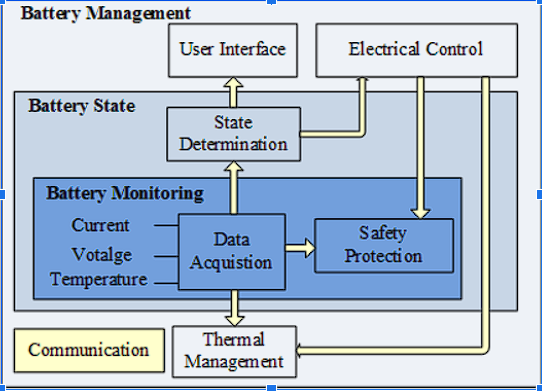
\includegraphics{bms.png}
    \caption{Sự mô tả về một hệ thống quản lý pin }
    \label{fig:enter-label}
\end{figure}

\vspace{7cm}
\subsection{Các phương pháp tối ưu và mô hình fog computing}
Như đã nói ở phần trước, thì sau khi đã đặc tả một số tính chất của hệ thống giám sát pin xe điện gồm: trạng thái sạc - SOC, trạng thái sức khỏe - SOH, vv… Cho nên phần sau đây sẽ mô tả thiết mở rộng với mô hình fog- computing và đưa ra một số phương án tối ưu cho các bài toán ở trên. 
\vspace{10cm}
\begin{figure}
    \centering
    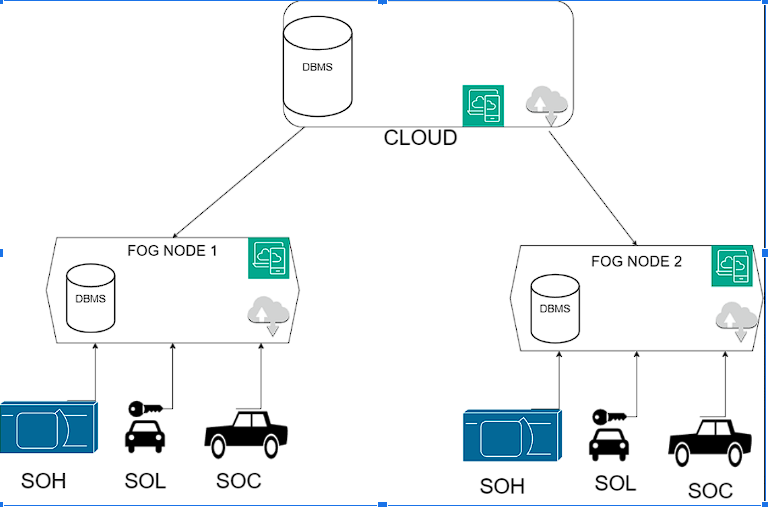
\includegraphics{fog-computing.png}
    \label{fig:enter-label}
\end{figure}
\vspace{5cm}

\textbf{Sử dụng phương pháp chọn khoảng thích hợp để giải quyết bài toán lưu trữ dữ liệu cho State of Charge(SOC) }
\begin{itemize}
    \item[--] Dữ liệu thu thập được về trạng thái sạc: Được biết công thức của State of Charge chứa đại lượng biến thiên theo thời gian t, cho nên nếu phải lưu trữ toàn bộ dữ liệu sẽ làm tốn bộ nhớ lưu trữ và quá trình truy xuất cũng trở nên chậm chạp hơn. 

    Cho nên thay vì ta phải lưu trữ toàn bộ dữ liệu bắn về liên tục (real-time), thì luận văn này đề xuất phương án lưu theo khoảng delta và ngưỡng chọn e, sao cho delta không vượt quá e, thì ta sẽ nhóm lại thành một cụm dữ liệu (cluster) để tối ưu việc lưu trữ.
    
\end{itemize}

\textbf{Sử dụng các mô hình học máy cho các bài toán về state of health và state of life}
\begin{itemize}
    \item [--] Support Vector Machine (SVM)(based model)
Máy vector hỗ trợ (Support Vector Machine - SVM) there một kỹ thuật tính toán mềm phổ biến và được sử dụng rộng rãi trong nhiều lĩnh vực. Nguyên tắc cơ bản của SVM là sử dụng ánh xạ phi tuyến cho việc ánh xạ dữ liệu trong một số lĩnh vực và áp dụng thuật toán tuyến tính trong không gian hàm.
    \item[--] Linear Regression (LR):
Các thuật toán hồi quy tuyến tính sẽ được áp dụng nếu đầu ra là một biến liên tục. Ngược lại, các thuật toán phân loại được áp dụng khi đầu ra được chia thành các phần như đạt/không đạt, tốt/trung bình/kém, vv. Chúng ta có các thuật toán hồi quy khác nhau hoặc phân loại hành vi, trong đó thuật toán hồi quy tuyến tính (Linear Regression - LR) là thuật toán hồi quy cơ bản. 
    \item[--] Ensemble Bagging (EBa):
Bagging (Bootstrap Aggregating) there một meta-algorithm trong học máy được thiết kế để tăng cường độ chính xác và độ chính xác của các thuật toán học máy trong phân loại thống kê và hồi quy. Nó cũng giảm phương sai và giúp tránh hiện tượng quá khớp. Bagging là một cách để giảm bớt sự không chắc chắn của ước lượng bằng cách tạo ra các dữ liệu bổ sung cho việc kiểm tra tập dữ liệu bằng cách tạo ra các biến thể sao chép để tạo ra các tập dữ liệu ban đầu khác nhau . Boosting là một chiến lược lặp lại dựa trên mô tả trước đó để điều chỉnh trọng số của quan sát.

 
\end{itemize}

\section{KẾ HOẠCH TRIỂN KHAI}
Trong thời gian sắp tới của luận văn, tôi dự định triển khai các công việc như sau:\\
- Chuẩn bị dữ liệu, chuẩn hóa bao gồm tiền xử lý nếu có\\
- Sử dụng các mô hình học máy để hỗ trợ đánh giá SOH, SOL\\
- Tối ưu lượng thông tin lưu trữ dữ liệu và đẩy lên cloud \\
- Sử dụng các phương pháp và hiện thực mô hình \\
- Kết hợp các mô hình cloud-computing \\
- Tổng hợp kết quả và viết báo cáo\\
- Thời gian thực hiện các công việc ở biểu đồ sau:

\begin{figure}[h]
\begin{center}
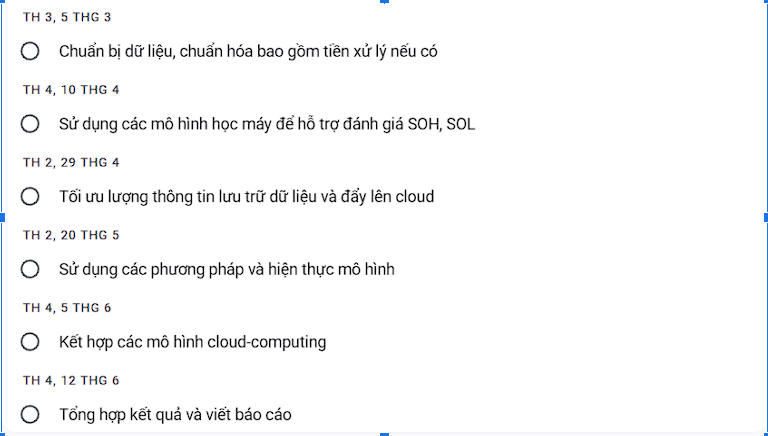
\includegraphics[width=5in]{plan.png}
\end{center}
\end{figure} 

\vspace{5cm}
\section{NỘI DUNG DỰ KIẾN CỦA LUẬN VĂN}

Nội dung báo cáo của luận văn dự kiến sẽ bao gồm các phần như sau:\\

\textbf{Chương 1: Giới thiệu}. Trong chương này sẽ trình bày một số vấn đề cơ bản của đề tài, nêu lên sự quan trọng của việc kiểm tra và giám sát thành phần trong xe điện trong lĩnh vực dữ liệu số hóa. Từ đó thấy được tầm quan trọng của đề tài để xác định rõ phạm vi và đối tượng nghiên cứu, hướng giải quyết của đề tài.
\\

\textbf{Chương 2: Các công trình nghiên cứu liên quan.} Trong chương này sẽ trình bày các công trình nghiên cứu liên quan. Tìm hiểu các phương pháp giải quyết vấn đề cũng như phạm vi, giới hạn của các nghiên cứu đó. Từ đó đánh giá tính khả thi của đề tài.\\

\textbf{Chương 3: Hiện thực và thử nghiệm mô hình. } Trong chương này sẽ trình bày chi tiết cách thức hiện thực của mô hình. Bao gồm các bước xây dựng và huấn luyện mô hình, sử dụng các mô hình và heuristic để giải quyết bài toán.\\

\textbf{Chương 4: Kết quả và đánh giá.} Trong chương này sẽ nêu ra các kết quả đạt được của mô hình, cũng như phương pháp đánh giá các kết quả đó.\\

\textbf{Chương 5: Kết luận.} Trong chương này sẽ tóm lại các ưu điểm và nhược điểm của mô hình và đưa ra các hướng nghiên cứu phát triển hệ thống trong tương lai.\\

\section{KẾT LUẬN}
Việc giám sát và quản lý pin đóng vai trò quan trọng trong đảm bảo hiệu suất, tuổi thọ và an toàn của hệ thống pin trên xe điện. Các công trình nghiên cứu liên quan đã tập trung vào các khía cạnh quan trọng như ước lượng trạng thái sạc và sức khỏe pin, chẩn đoán và tiên đoán lỗi, và quản lý thông minh của pin.\\

Để giám sát pin trên xe điện một cách hiệu quả, cần phải có hệ thống quản lý pin (BMS) thông minh và chính xác. BMS sẽ thu thập dữ liệu về trạng thái pin như trạng thái sạc, nhiệt độ, điện áp và dòng điện, sau đó phân tích và đưa ra các quyết định để bảo vệ pin và tối ưu hóa hiệu suất sử dụng năng lượng.\\

Công nghệ và phương pháp giám sát pin ngày càng phát triển, bao gồm sự kết hợp của cảm biến, hệ thống ghi dữ liệu, trí tuệ nhân tạo và học máy. Các phương pháp này giúp ước lượng trạng thái sạc và sức khỏe pin một cách chính xác, phát hiện và chẩn đoán lỗi một cách nhanh chóng, và dự đoán tuổi thọ còn lại của pin.\\

Thông qua việc nghiên cứu và áp dụng các công trình liên quan, có thể nâng cao hiệu suất và tuổi thọ của pin trên xe điện, giúp tăng khả năng di chuyển và đáp ứng nhu cầu của người sử dụng. Đồng thời, việc giám sát pin cũng đóng vai trò quan trọng trong việc đảm bảo an toàn và hạn chế các vấn đề liên quan đến pin như quá nhiệt, quá điện áp hoặc quá dòng điện.\\

Tổng quan, đề tài "Giám sát pin trên xe điện" là một lĩnh vực nghiên cứu quan trọng và đầy triển vọng, đóng góp vào sự phát triển của công nghệ pin và xe điện hiệu quả và bền vững.\\

\begin{thebibliography}{19}

\bibitem{H. Truong:Rahman:Shenoy:2018} 
H. Truong, S. Rahman, và P. S. Shenoy (2018),
Battery Management Systems in Electric and Hybrid Vehicles.

\bibitem{Benmouiza}
A. Benmouiza và A. Chandra,
State of Charge Estimation of Lithium-Ion Batteries in Electric Vehicles: A Review

\bibitem{Y. Hu}
Y. Hu, L. Wang, và H. Gao,
Real-Time State of Health Estimation for Lithium-Ion Batteries in Electric Vehicles

\bibitem{Y. Li}
Y. Li và C. Mi.,
Data-Driven Fault Diagnosis and Prognosis of Lithium-Ion Batteries in Electric Vehicles

\bibitem{X. Hu}
X. Hu, Y. Li, và C. Mi.,
Intelligent Battery Management and Control for Electric Vehicles

\bibitem{Rui Xiong}
Rui Xiong, Kui Zhang,
Design and implementation of a Battery Big Data Platform Through Intelligent Connected Electric Vehicles

\bibitem{Cheng:2011}
Cheng, K.W.E.; Divakar, B.P.; Wu, H.J.; Ding, K.; Ho, H.F,
Battery-Management System (BMS) and SOC development for electrical vehicles,
\textbf{IEEE Trans. Veh. Technol}, 60, 76--88, 2011

\bibitem{Tipping:2000}
Tipping, M.E,
The Relevance Vector Machine. Advances in Neural Information Processing Systems,
\textbf{MIT Press: Cambridge, MA, USA}, 12, 287--289, 2000

\bibitem{Widodo:2011}
Widodo, A.; Shim, M.C.; Caesarendra, W.; Yang, B.-S,
Intelligent prognostics for battery health monitoring based on sample entropy,
\textbf{Expert Syst. Appl}, 38, 11763--11769, 2011

\bibitem{Chao:2011}
Chao, K.H.; Chen, J.W,
State-of-health estimator based on extension theory with a learning mechanism for lead-acid batteries,
\textbf{Expert Syst. Appl}, 38, 15183--15193, 2011

\bibitem{Moo:2009}
Ng, K.S.; Moo, C.S.; Chen, Y.P.; Hsieh, Y.C,
Enhanced coulomb counting method for estimating state-of-charge and state-of-health of lithium-ion batteries,
\textbf{Appl. Energy}, 86, 1506--1511, 2009

\bibitem{}
State of Charge (SOC) Determination,
\textbf{http://www.mpoweruk.com/soc.htm},
232, 2011

\end{thebibliography}
\end{document}